\documentclass{ieeeaccess}
\usepackage{cite}
\usepackage{amsmath,amssymb,amsfonts}
% The IEEE Access class selects Times/Helvetica/Courier in T1 encoding (see the
% class font definitions); load the matching font packages so those shapes are
% defined instead of being substituted with (wider) Computer Modern.
\usepackage[T1]{fontenc}
\usepackage{mathptmx}
\usepackage[scaled=.92]{helvet}
\usepackage{courier}
\usepackage{algorithmic}
\usepackage{algorithm}
\usepackage{graphicx}
\usepackage{textcomp}
\usepackage{url}
\usepackage{booktabs}
\usepackage{multirow}
\def\BibTeX{{\rm B\kern-.05em{\sc i\kern-.025em b}\kern-.08em
    T\kern-.1667em\lower.7ex\hbox{E}\kern-.125emX}}
% The IEEE Access class sets \xfigwd only inside its custom \Figure command; define a
% default so standard figure environments work with the class caption macro.
\providecommand{\xfigwd}{0pt}
% ieeeaccess.cls uses \if@biographyTOCentrynotmade in its biography environments but never
% declares the flag; declare it here so IEEEbiographynophoto compiles (author bios at the end).
\makeatletter
\newif\if@biographyTOCentrynotmade
\@biographyTOCentrynotmadetrue
\@ifundefined{c@biography}{\newcounter{biography}}{}
\makeatother
\begin{document}
\history{Date of current version August 2026.}
\doi{10.1109/ACCESS.2026.DOI}

%\title{How Far Can a PSRAM-less ESP32 Go? A TinyML Deployment Study for WiFi CSI Human Activity Recognition}
%\title{Feasibility and Deployment Analysis of TinyML-based WiFi Human Activity Recognition on Resource-Constrained ESP32}
% R2-1: reviewer asked to replace the acronyms TinyML and ESP32 in the title with words.
\title{Feasibility and Deployment Analysis of Tiny Machine Learning for WiFi-Based Human Activity Recognition on a Resource-Constrained Microcontroller}
% E5/E6: author list and corresponding author restored to match the original submission
% (Malik, Ahmad, Kim; Kim corresponding). The list is identical to the submitted version, so
% no Request-for-Byline-Change form is required.
\author{
\uppercase{Annas W. Malik}\authorrefmark{1},
\uppercase{Muhammad Ahmad}\authorrefmark{1},
\uppercase{Ki-Il Kim}\authorrefmark{2}
}

\address{
\authorrefmark{1}Faculty of Information Technology \& Computer Science, University of Central Punjab, Lahore, 54000, Pakistan.\\
\authorrefmark{2}Department of Computer Science and Engineering, Chungnam National University, Daejeon, 34134, Korea.
}

\tfootnote{This work was supported by Korea Institute of Planning and Evaluation for Technology in Food, Agriculture, and Forestry(IPET) through the Agriculture and Food Convergence Technologies Program for Research Manpower development, funded by the Ministry of Agriculture, Food and Rural Affairs(MAFRA)(project no. RS-2024-00397026).}

\markboth
{Annas W. Malik \headeretal}
{Annas W. Malik \headeretal}

\corresp{Corresponding author: Ki-Il Kim (e-mail: kikim@cnu.ac.kr).}

%\begin{abstract}
%WiFi Channel State Information (CSI) is a useful signal for device-free human activity recognition (HAR), and a growing number of studies move the inference onto the cheap microcontroller-class radios themselves so the technology can be deployed at scale. Almost all of that on-device work, however, targets the more capable ESP32-S3 with external PSRAM, or it uses the microcontroller only as a CSI collector and runs the model elsewhere. The cheapest, most common, and weakest member of the family, the classic ESP32 with no PSRAM and only about 150 kilobytes of usable contiguous internal SRAM, has not been characterized as an inference target for CSI HAR. This paper provides that characterization and reaches a two-part conclusion: on this device, getting a model to run is not the bottleneck, but recognizing an unseen person is. For two public datasets (UT-HAR and CSI-HAR) we train and quantize a graded set of models, from classical learners (Decision Tree, Random Forest, and a small multilayer perceptron on handcrafted statistics) through a tiny-CNN width sweep up to five standard deep architectures (convolutional, recurrent, attention, Kolmogorov-Arnold, and state-space), reporting accuracy, model complexity, 8-bit conversion feasibility, and on-device fit. On the deployment side the board is more capable than assumed. A convertibility wall blocks only the recurrent and state-space families, which do not convert to the TensorFlow Lite for Microcontrollers builtin operator set on either dataset. By flashing every convertible model to the board we find that a full deep convolutional network and a convolution-augmented Transformer both run on the bare classic ESP32 within 10 to 54 kilobytes of tensor arena, alongside the classical learners and the tiny CNNs (int8 models of 9 to 38 kilobytes, 9 to 68 milliseconds per inference at 240\,MHz). There is no general memory wall, which corrects a common assumption. The binding constraint is accuracy on a new person. Under a subject-independent leave-one-user-out protocol on CSI-HAR, the same models that score 69 to 96\% on a random split, which leaks each user across the train and test sets, fall to 41 to 63\%, a mean drop of 29 percentage points. The contribution is a fair, reproducible deployment map of the most constrained commodity WiFi microcontroller, and the evidence that its open problem is cross-subject generalization rather than fitting the model on the chip, with all code, models, and measurement firmware released.
%\end{abstract}

% R2-2: abstract reorganized (background, gap, method, results, conclusion) and expanded to
% include the measured energy, the live pipeline, and the many-user CSI-Bench check; acronyms
% expanded at first use (R1-5, R2-3). Previous abstract kept above (commented) for provenance.
\begin{abstract}
WiFi channel state information (CSI) enables device-free human activity recognition (HAR) without cameras or wearable sensors, and moving the inference onto low-cost microcontrollers would make such sensing deployable at scale. Existing on-device studies, however, target the ESP32-S3, which adds external pseudo-static random-access memory (PSRAM), or use the microcontroller only to collect CSI. The cheapest and most constrained member of the family, the classic ESP32 without PSRAM (about 150 kilobytes of usable static random-access memory), has not been characterized as an inference target. This paper provides that characterization. On two public datasets (UT-HAR and CSI-HAR) we train and quantize a graded set of models, from classical learners and tiny convolutional neural networks (CNNs) to five deep architectures, and measure each on the physical device for conversion feasibility, memory footprint, latency, and energy. By flashing every convertible model to the board we find that memory is not the bottleneck: a deep CNN and a convolution-augmented Transformer both run within a 10 to 54 kilobyte tensor arena, whereas only recurrent and state-space models fail to convert to the microcontroller runtime. Per-inference energy is measured directly with an INA219 current sensor, and a 30-minute live capture-to-label pipeline runs on the device with no lost windows. The binding constraint is cross-subject generalization: under subject-independent leave-one-user-out (LOUO) evaluation, accuracy falls by an average of 29 percentage points, a gap we reproduce on the 35-user CSI-Bench dataset. On-device CSI HAR on commodity microcontrollers is therefore limited by subject generalization rather than by chip memory.
\end{abstract}

% R2-4: keywords no longer repeat terms present in the title (human activity recognition, WiFi,
% tiny machine learning, microcontroller); replaced with terms that broaden the article's reach.
\begin{keywords}
Channel state information, cross-subject generalization, edge computing, ESP32, model quantization, on-device machine learning, TensorFlow Lite for Microcontrollers.
\end{keywords}

\titlepgskip=-15pt

\maketitle

% R1-2, R1-5, R2-3: abbreviations defined once, in order, so no acronym is used undefined.
% Uses IEEEdescription so the list flows and breaks across columns/pages cleanly.
\section*{Nomenclature}
\begin{IEEEdescription}[\IEEEsetlabelwidth{PSRAM}]
\item[CNN] Convolutional Neural Network.
\item[CSI] Channel State Information.
\item[DT] Decision Tree.
\item[GRU] Gated Recurrent Unit (BiGRU: bidirectional GRU).
\item[HAR] Human Activity Recognition.
\item[KAN] Kolmogorov-Arnold Network.
\item[LOUO] Leave-One-User-Out (subject-independent evaluation in which the test user is absent from training).
\item[MCU] Microcontroller Unit.
\item[ML] Machine Learning.
\item[MLP] Multilayer Perceptron.
\item[NPU] Neural Processing Unit.
\item[PSRAM] Pseudo-Static Random-Access Memory (external RAM absent on the classic ESP32).
\item[RF] Random Forest.
\item[SIMD] Single Instruction, Multiple Data (vector kernels).
\item[SoC] System on Chip.
\item[SRAM] Static Random-Access Memory (on-chip).
\item[SSM] State-Space Model.
\item[TFLM] TensorFlow Lite for Microcontrollers.
\end{IEEEdescription}

\section{Introduction}
\label{sec:introduction}
\PARstart{W}{iFi} Channel State Information (CSI) has become a practical signal for device-free human activity recognition (HAR). Because CSI is reflected and scattered by a moving body, a receiver can infer activity without a camera and without any wearable on the user, which is attractive for privacy-sensitive settings such as homes, clinics, and assisted-living facilities. The release of commodity CSI extraction tools \cite{halperin2011csi} and a decade of deep-learning architectures \cite{ma2019wifi,yang2023sensefi} have pushed in-distribution accuracy on the standard benchmarks above 98\%.

A second trend is just as important for real deployment: moving the inference onto the cheap radios themselves. The Espressif ESP32 family, dual-core microcontrollers with WiFi and a few hundred kilobytes of RAM that cost under ten US dollars, is a widespread platform for this. Running the model on the device avoids streaming raw CSI to a server, removes the associated privacy and bandwidth costs, and is what would make WiFi sensing deployable at the scale of a light switch. Recent work has shown that compact convolutional and recurrent models can be quantized to 8-bit precision and run on ESP32-class hardware \cite{hernandez2025tools,espfihar2026}.

These two trends meet at a question that the literature has not answered. The published on-device CSI studies target the ESP32-S3, which carries several megabytes of external PSRAM and therefore relaxes the memory constraint, or they use the microcontroller purely as a CSI collector and run the classifier on a gateway or a server. The classic ESP32, the original and still the most widely deployed member of the family, has no PSRAM and exposes only a few hundred kilobytes of internal SRAM, of which a single contiguous block of roughly 150 kilobytes is realistically available to a model at runtime once the radio stacks are disabled. It is also, by Espressif's own ranking, the weakest CSI source in the family. This cheapest and most constrained device is precisely the one a cost-sensitive deployment would choose, and it has not been characterized as an inference target for CSI HAR. A practitioner who holds a bare classic ESP32 has no evidence about what, if anything, will actually run on it.

\subsection{Contributions}
\label{sec:contributions}
This paper answers that question with a deployment-characterization study rather than a new model. It reaches a two-part result: the bare classic ESP32 runs far more than expected, so for the model families and public datasets we tested, memory feasibility was not the limiting deployment factor, and cross-subject generalization emerged as the dominant accuracy limitation. We present the latter as an exploratory case-study finding on a small dataset, not a universal claim. The contributions are:
\begin{enumerate}
    \item A \textbf{deployability frontier} for WiFi CSI HAR on the PSRAM-less classic ESP32, spanning classical learners, tiny neural networks, and five standard deep architectures, each reported with accuracy, complexity, 8-bit conversion feasibility (whether the trained model can be translated into the integer operator set the microcontroller runtime supports), model size, and on-device fit.
    \item An \textbf{on-device characterization of which deep architectures actually deploy}, measured by flashing each to the board: the convolutional and Transformer models convert and run on the bare device, the recurrent and state-space models do not convert (an export-pipeline compatibility boundary), and the Kolmogorov-Arnold model converts but fails at operator preparation. This corrects the common assumption that deep models cannot fit such a device.
    \item A \textbf{positive deployability result}: classical learners and tiny convolutional networks both fit the device, the former trivially and the latter as int8 models of 9 to 38 kilobytes, and we quantify the accuracy each retains on two datasets.
    \item An exploratory characterization of the \textbf{cross-subject generalization gap} on a three-user dataset, which on that data exceeds the deployment constraint (presented as a case study, not a universal claim). On this three-user CSI-HAR dataset, under a subject-independent leave-one-user-out (LOUO) protocol, in which the model is tested on a user who is entirely absent from training, six models drop by a mean of 29 percentage points (the best from 96\% to 63\%) relative to a random subject-overlapping split in which the same users appear in train and test. The deployment barriers on the PSRAM-less ESP32 are less restrictive than commonly assumed; our experiments suggest that generalizing to an unseen person may be the more significant challenge.
    \item A \textbf{reproducible artifact set}: the training and quantization notebook, the exported int8 models and classical models, the emlearn C export of the trees (emlearn compiles a trained tree or forest into plain branch-only C code), and the ESP32 measurement firmware and protocol.
\end{enumerate}

\subsection{Scope and honest positioning}
\label{sec:scope}
This paper is a deployment-characterization study, not a new-model paper. We do not propose a novel architecture or claim a new accuracy record; the models we use are standard, and UT-HAR accuracy is already saturated. The contribution is instead an empirical map of what actually converts, allocates, and runs on the bare classic ESP32, measured on the physical device, together with the finding that locates the open problem in cross-subject generalization rather than in fitting the model on the chip. As detailed in Section~\ref{sec:related}, no prior study characterizes inference on the bare, PSRAM-less classic ESP32 across a graded classical-to-deep model set, which is the gap we fill; we regard a fair, reproducible deployment map, including the negative findings, as a useful contribution for practitioners.

\section{Related Work}
\label{sec:related}

\subsection{Model Families for WiFi CSI HAR}
The move from hand-crafted features to end-to-end learning produced a sequence of architectures evaluated on a stable set of benchmarks. ABLSTM \cite{chen2019ablstm} introduced attention-augmented bidirectional recurrence; THAT \cite{li2021that} replaced recurrence with a two-stream convolution-augmented Transformer; the SenseFi library \cite{yang2023sensefi} standardized training and evaluation across UT-HAR, NTU-Fi, and Widar and reports strong baselines (ResNet-18 at 98.11\% on UT-HAR). Recent work emphasizes lightweight and complementary-feature models, including a pruned attention-GRU \cite{khan2025lightweight} and the amplitude-and-phase PA-CSI model \cite{pacsi2025}. Two newer families are also relevant to our deep tier. Kolmogorov-Arnold Networks \cite{kanorig2024} replace the fixed activations of a multilayer perceptron with learnable univariate functions on the network edges; they have reached WiFi HAR at the gateway, for example in neurosymbolic CNN-Transformer healthcare models \cite{neurosym2025}, but have not been measured on a microcontroller. State-space models such as Mamba \cite{gu2023mamba} model long sequences with a linear-time recurrence and have been applied to CSI HAR on the GPU by TF-Mamba \cite{tfmamba2025} and bidirectional-Mamba HAR \cite{bimamba2025}. Almost all of this work optimizes accuracy on server-class hardware, on which the on-chip memory constraint studied here does not apply, and whether the recurrent, state-space, or Kolmogorov-Arnold families convert to and fit the bare classic ESP32 for CSI HAR has not been measured.

\subsection{On-Device and TinyML WiFi Sensing}
Outside the deep-learning literature, classical learners remain the workhorses of microcontroller deployment because their footprint and inference cost are small and predictable: decision trees and ensembles compile to compact branch-only C through tools such as emlearn \cite{emlearn}, and prior CSI work shows that classical models on statistical features reach useful accuracy off-device \cite{mdpiclassical}. TinyML neural-architecture-search studies such as TinyTNAS \cite{tinytnas2024} and MicroNAS \cite{micronas2025} target microcontroller HAR but for inertial sensors rather than CSI, and Suwannaphong \emph{et~al.}~\cite{suwannaphong2025tinyml} optimize TinyML transformer and Mamba models for 32 to 64 kilobytes of RAM but for indoor localization. For on-device WiFi sensing specifically, standalone ESP32 CSI collection was popularized by Hernandez and Bulut \cite{hernandez2020lightweight,hernandez2023edge}, whose survey stresses that a complete edge system must handle live capture, windowing, and preprocessing, not inference alone. The most directly comparable prior work that runs inference \emph{on} the chip is Lenka and Chakraborty \cite{lenka2024wisdom}, whose Wisdom framework benchmarks compressed int8 DNN inference on a PSRAM-less ESP32-C3 (single-core RISC-V), and Armenta-Garcia \emph{et~al.}~\cite{hernandez2025tools}, who deploy a quantized DenseNet on the PSRAM-equipped ESP32-S3 (92.43\%, 232\,ms, 127\,kB).

\emph{Distinction from the closest prior ESP32 work.} Because several studies are loosely described as ``CSI HAR on the ESP32,'' we separate the acquisition device from the inference device throughout (Table~\ref{tab:priorcompare}) and state the distinction explicitly for the two works most likely to be read as prior art. Sahoo \emph{et~al.}~\cite{sahoo2023realtime} build a real-time smart-home detector around ESP32 CSI but run the classifier on an edge/host layer, so the ESP32 is the sensor, not the inference target. MambaLite-Micro \cite{mambalite2025} is a state-space inference engine evaluated on the ESP32-S3 and STM32H7 for keyword spotting and inertial (accelerometer) HAR in floating point with a hand-written engine; it does not address WiFi CSI, the PSRAM-less classic ESP32, or the TensorFlow Lite Micro toolchain. Likewise STAR \cite{star2025} runs its model on a Rockchip RV1126 neural processing unit and uses the ESP32-S3 only as the CSI front end, and the ESP-Fi HAR work \cite{espfihar2026} provides an ESP32-C3-collected dataset with a host-side benchmark. Across this line, 8-bit integer quantization is effectively mandatory for the ESP32 memory budget \cite{greensensing2026}, and the non-convertibility of recurrent and dynamic operators through the standard export route is documented in the TensorFlow and TensorFlow Lite Micro issue trackers \cite{tfissue36688,tflmissue907}, which we corroborate here for CSI models. Against this background, the contribution of this paper is a systematic, measured int8 inference-deployability frontier on a PSRAM-less ESP32-WROOM-32 across classical, tiny, and compact deep CSI-HAR models, together with a live acquisition-to-prediction demonstration on the same board, none of which the prior work provides.

\begin{table*}[t]
\caption{On-device WiFi CSI sensing across the ESP32 family, separating the CSI acquisition device from the inference device to avoid conflating the two. ``On-chip'' is whether the WiFi-sensing inference runs on the ESP32 itself (as opposed to a host or a separate accelerator); ``Live'' is on-device live CSI capture; ``Prep.'' is on-device preprocessing. Y = yes, N = no, P = partial, n/r = not reported, n/a = not applicable. Values are each study's own reports on its own setup and are not directly comparable; the point of the table is what each system actually runs on-chip. For this work, Live and Preproc.\ are Y on the strength of the 30-minute on-device live capture, windowing, normalization, and quantization run (Section~\ref{sec:results-live}); live classification accuracy is not measured because the deployed model is out-of-domain. The latency range is at 240\,MHz, the operating point used for all on-device results.}
\label{tab:priorcompare}
\centering
\footnotesize
\setlength{\tabcolsep}{3.5pt}
\resizebox{\textwidth}{!}{%
\begin{tabular}{lllcccllccll}
\toprule
Work & Acq.\ dev. & Inference dev. & On-chip & Live & Prep. & Models & Quant. & PSRAM & RAM & Latency & Energy \\
\midrule
Hernandez \& Bulut '20 \cite{hernandez2020lightweight} & classic ESP32 & host & N & Y & N & CSI collection & n/a & N & n/r & n/r & n/r \\
Sahoo \emph{et~al.}\ '23 \cite{sahoo2023realtime} & ESP32 & edge/host & N & Y & P & activity det. & n/r & N & n/r & real-time & n/r \\
ESP-Fi HAR \cite{espfihar2026} & ESP32-C3 & host & N & N & N & CNN bench. & n/r & N & n/a & n/a & n/a \\
STAR \cite{star2025} & ESP32-S3 & RV1126 NPU & N & Y & n/r & light CNN & int8 & Y & n/r & sub-sec & n/r \\
Lenka \& Chakraborty '24 \cite{lenka2024wisdom} & ESP32-C3 & ESP32-C3 & Y & Y & Y & compressed DNN & int8 & N & $\sim$400\,kB & rep. & rep. \\
Armenta-Garcia \emph{et~al.}\ '25 \cite{hernandez2025tools} & ESP32-S3 & ESP32-S3 & Y & Y & Y & DenseNet & int8 & Y & 127\,kB & 232\,ms & n/r \\
\textbf{Proposed study} & \textbf{classic ESP32} & \textbf{classic ESP32} & \textbf{Y} & \textbf{Y} & \textbf{Y} & \textbf{classical+tiny+deep} & \textbf{int8+emlearn} & \textbf{N} & \textbf{8--54\,kB} & \textbf{9--321\,ms} & \textbf{INA219} \\
\bottomrule
\end{tabular}}
\end{table*}

\textit{Gap.}~No prior study characterizes the bare, PSRAM-less classic ESP32 as an inference target for WiFi CSI HAR, nor maps which models across the classical, tiny, and deep spectrum actually fit it. This paper fills that gap.

\begin{figure*}[!t]
\centering
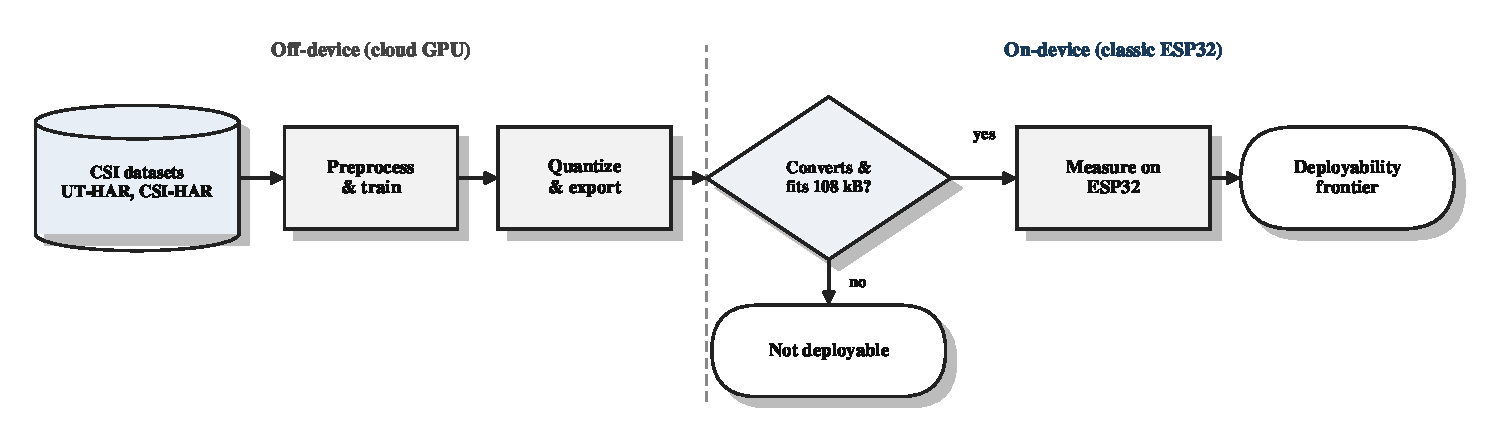
\includegraphics[width=0.9\textwidth]{fig_pipeline.pdf}
\caption{System and measurement pipeline. Models are trained and quantized off-device on a cloud GPU, then exported as int8 TensorFlow Lite (neural models) or emlearn C (classical models), deployed on the bare classic ESP32, and measured for on-device latency and peak RAM. Convertibility and on-device allocation are evaluated at the deploy stage, and the result is the deployability frontier.}
\label{fig:pipeline}
\end{figure*}

\section{Models Under Study}
\label{sec:models}
The frontier spans three tiers (Figure~\ref{fig:pipeline}), all consuming the same input representation. A CSI window is a real-valued tensor $\mathbf{X}\in\mathbb{R}^{T\times F}$ with $T$ time steps and $F$ per-step features. We downsample the time axis to $T=64$ by uniform index selection, which costs almost no accuracy on UT-HAR while shrinking activations, and we standardize each window.

\subsection{Classical learners}
For the classical tier, each window is summarized by five statistics computed over time for every feature dimension: mean, standard deviation, minimum, maximum, and range, giving a compact $F\times 5$ vector that is cheap to compute on a microcontroller. On these features we train a depth-limited Decision Tree, a Random Forest of twenty depth-limited trees, and a small multilayer perceptron with one hidden layer of thirty-two units. The Random Forest settings are deliberately small for the target: twenty trees at a maximum depth of ten keep the total node count and the emlearn C footprint within a few kilobytes of flash, and on our data accuracy saturates well before this size, so a larger forest would only add footprint without a matching accuracy gain. Trees and forests are exported to branch-only C with emlearn \cite{emlearn}, which reproduces the trained decision structure as a nested sequence of threshold comparisons. Because the exported code branches on the same split thresholds learned by scikit-learn, the decision path, and therefore the predicted label, is identical to the scikit-learn model for any input represented consistently with training; parity holds by construction rather than as an empirical approximation. The one caveat we flag is representation: emlearn's default integer feature path stores thresholds in a fixed-point format, so the on-device feature statistics must be computed and scaled in the same fixed-point domain as the exported thresholds for the decision paths to coincide. We therefore report the off-device accuracy for these models and compute the on-device features in the matching representation.

\subsection{Tiny neural networks}
The tiny tier comprises a tiny multilayer perceptron (one hidden layer of thirty-two units on the flattened window) and a tiny-CNN width sweep with 8, 16, and 32 channels in the first convolutional block. Each tiny CNN has two 1D convolutional blocks, global average pooling, and a dense classifier. These models are trained in floating point and then quantized to int8.

\subsection{Deep architectures}
The deep tier comprises five standard families: a 1D convolutional network, a bidirectional gated recurrent unit, a convolution-augmented Transformer following the spirit of THAT \cite{li2021that}, a Chebyshev Kolmogorov-Arnold network \cite{kanorig2024}, and a lightweight diagonal state-space model \cite{gu2023mamba}. They are sized to comparable parameter budgets and contribute the upper, large-model part of the frontier. To keep the comparison fair and the results verifiable, the deep tier uses the same training, 8-bit quantization, and on-device measurement protocol as the classical and tiny tiers (Section~\ref{sec:setup}); the deep-tier training notebook and the resulting int8 models are part of the released artifact set, so every deep-tier value is reproducible from the release rather than taken on trust. Table~\ref{tab:params} lists the parameter count of each deep model; the five families sit within the same order of magnitude (42 to 91\,K), so the on-device comparison is not confounded by grossly different capacity.

\begin{table}[t]
\caption{Parameter counts of the five deep architectures (float model, UT-HAR configuration). The families are deliberately sized to comparable budgets so that deployability, not capacity, is what the comparison isolates.}
\label{tab:params}
\centering
\footnotesize
\begin{tabular}{lc}
\toprule
Deep model & Parameters \\
\midrule
CNN              & 91.0\,K \\
BiGRU            & 68.6\,K \\
Transformer      & 62.8\,K \\
Chebyshev-KAN    & 79.1\,K \\
Lightweight-SSM  & 41.7\,K \\
\bottomrule
\end{tabular}
\end{table}

\section{Experimental Setup}
\label{sec:setup}

\subsection{Datasets}
We use two public datasets for the core study, a third to confirm the frontier, and a fourth, many-user corpus to check the generalization gap; Table~\ref{tab:datasets} summarizes their receivers, subcarrier counts, subjects, and role. Together they span three CSI receiver families (Intel 5300, the Broadcom chip read by Nexmon, and Atheros) plus the in-the-wild CSI-Bench, and subject counts from three to thirty-five, which is the diversity of devices and environments available from public data; we did not record a new environment ourselves, a limitation we return to in Section~\ref{sec:discussion}. UT-HAR \cite{yousefi2017uthar}, obtained through the SenseFi loaders \cite{yang2023sensefi}, is the most widely used public CSI HAR benchmark (Intel 5300, seven activities, native $T=250$, $F=90$). CSI-HAR \cite{csihardataset} is a commodity single-antenna dataset of seven activities recorded by three users with twenty samples each, collected with a Raspberry Pi 4 and the Nexmon CSI tool on an 802.11ac link (variable-length sequences over 52 subcarriers). UT-HAR uses its standard split with three seeds; CSI-HAR is evaluated subject-independently with leave-one-user-out (each of three folds trains on two users and tests on the held-out third), which avoids the subject overlap of a random within-user split and is the standard rigour for HAR generalization. As an independent frontier check we also use NTU-Fi\_HAR \cite{yang2023sensefi} (six whole-body activities, three antennas, 114 subcarriers), reported for accuracy only. The fixed splits for UT-HAR and NTU-Fi\_HAR are at the window level and are not subject-partitioned, so their high accuracy reflects in-distribution performance; we therefore treat them as saturated in-distribution benchmarks and draw every cross-subject conclusion only from CSI-HAR. Two preprocessing details matter for reproducibility. Each window is z-score normalized by a single scalar mean and standard deviation computed jointly over its time and subcarrier axes (not per subcarrier), so it is normalized only by its own statistics and there is no fitting across windows and hence no train-test leakage in either protocol. Variable-length recordings are resampled along time to a common $T=64$ by linear index subsampling; an ablation over $T\in\{32,64,128,192\}$ under leave-one-user-out gives 57.6, 59.5, 55.2, and 54.5\% for the 16-channel tiny CNN on CSI-HAR, so $T=64$ is at or near the optimum. Under leave-one-user-out, every fitted quantity that could leak the held-out user (the int8 calibration windows and any tuned hyperparameter) is taken from that fold's training users only, and hyperparameters are in fact fixed a priori and not tuned per fold, so no held-out-user information enters model selection.

\begin{table}[t]
\caption{Datasets used, spanning three CSI receiver families and subject counts from three to thirty-five. ``Subjects'' is n/r where the public split is at the window level and not subject-labelled. CSI-Bench is used only for the many-user cross-subject check (Section~\ref{sec:results-gap}); NTU-Fi\_HAR only for the frontier check (Supplementary Material).}
\label{tab:datasets}
\centering
\footnotesize
\setlength{\tabcolsep}{3pt}
\resizebox{\columnwidth}{!}{%
\begin{tabular}{lllcl}
\toprule
Dataset & Receiver & Subcarr. & Subj. & Role here \\
\midrule
UT-HAR \cite{yousefi2017uthar}      & Intel 5300         & 3$\times$30  & n/r & frontier, quant. \\
CSI-HAR \cite{csihardataset}        & Raspberry Pi (Nexmon) & 52        & 3   & on-device, cross-subj. \\
NTU-Fi \cite{yang2023sensefi}       & Atheros            & 3$\times$114 & n/r & frontier check \\
CSI-Bench \cite{csibench2025}       & in-the-wild WiFi   & varies      & 35  & cross-subj.\ check \\
\bottomrule
\end{tabular}}
\end{table}

\subsection{Training and quantization}
All neural models are trained with one shared pipeline: Adam at learning rate $10^{-3}$, batch size 64, for 40 epochs, with sparse categorical cross-entropy on logits. These two settings were fixed by a grid sweep on CSI-HAR over learning rates $\{10^{-2},10^{-3},10^{-4}\}$ and batch sizes $\{32,64,128\}$ for the CNN, Transformer, and bidirectional GRU; learning rate $10^{-3}$ with batch size 64 was the optimum for both the CNN (96.4\%) and the Transformer (94.0\%) and within one point of the best for the GRU, so we adopt it throughout and release the full grid with the notebook. Classical learners are trained over three seeds and we report mean and standard deviation. Each trained network is converted to 8-bit integer precision with TensorFlow Lite using post-training static quantization calibrated on 300 representative windows drawn from that fold's training users only (never the held-out user); we attempt full int8 input and output first and fall back if an operator forbids it. We record, for each model, whether conversion succeeds and the resulting model size. Off-device training and quantization run on a cloud GPU; the released notebook reproduces every off-device number.

\subsection{On-device platform and measurement}
\begin{figure}[tbp]
\centering
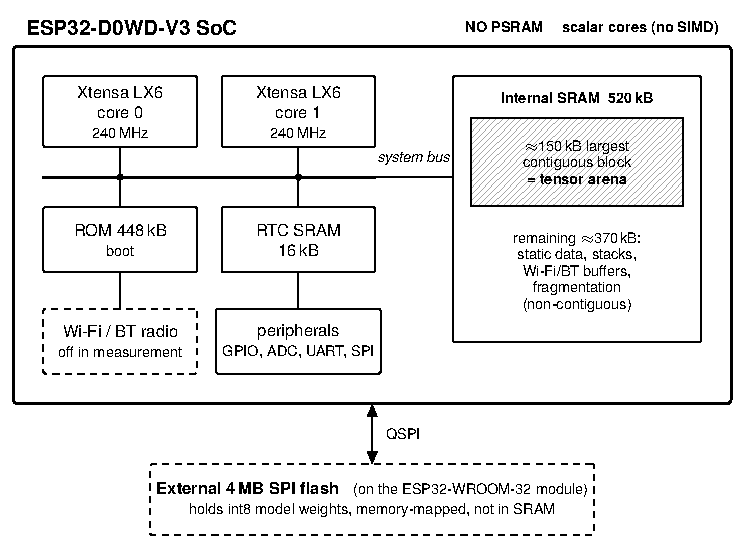
\includegraphics[width=\columnwidth]{fig_esp32_internal.pdf}
\caption{Internal components of the classic ESP32 (ESP32-D0WD-V3) relevant to on-device inference. Two scalar Xtensa LX6 cores at 240\,MHz (no vector unit) execute the model; the 520\,kB internal SRAM holds all int8 activations, and its largest free contiguous block (about 150\,kB with the radio stacks disabled) is the tensor arena that a model must fit. The quantized model weights live in the external 4\,MB flash, not in SRAM. There is no PSRAM. The on-chip WiFi/BT radio is disabled during our inference measurements. Regions and sizes are those measured on the board (Section~\ref{sec:setup}).}
\label{fig:board}
\end{figure}
The deployment target is a commodity classic ESP32 on an ESP32-WROOM-32 module (Figure~\ref{fig:board}; ESP32-D0WD-V3, silicon revision v3.1 per \texttt{esptool}, dual-core Xtensa LX6 at 240\,MHz, 520\,kB internal SRAM, \emph{no PSRAM}, 4\,MB flash) running TensorFlow Lite for Microcontrollers. For reproducibility the firmware is built with ESP-IDF v5.1 (its bundled Xtensa GCC 12.2.0), TFLM is provided by the \texttt{esp-tflite-micro} component, and models are quantized off-device with TensorFlow 2.19; unless stated otherwise the firmware uses the default optimization level at 240\,MHz. With the radio stacks disabled, a single contiguous block of roughly 150\,kB is available to a model at runtime (the firmware reports about 152\,kB), and this is the binding budget. For each convertible model we attempt allocation and, on success, measure latency as the mean over 1000 hardware-timer invocations, peak RAM as the interpreter's tensor arena (\texttt{arena\_used\_bytes()} after \texttt{AllocateTensors}, the figure that must fit the budget), and flash as the model byte array. The quantized weights live in flash and are not part of the SRAM budget, so peak RAM in our tables is the measured arena, not an estimate. Energy is measured directly with an INA219 current sensor in series with the 5\,V board input, isolating active inference from the idle baseline with a GPIO marker driven high during each inference; because the sensor resolves mean power over a multi-millisecond inference but not sub-millisecond transients, the microsecond-scale classical inference is reported as below its resolution rather than as a precise value. We do not use ESP32-S3 measurements to bound the classic ESP32, and any datasheet current we cite for context (30 to 68\,mA in modem-sleep at 240\,MHz with the radio off \cite{esp32datasheet}) is given as a range, not a single value. Decision trees and forests are deployed as emlearn C and timed the same way; the firmware, flash offsets, and capture protocol are released with the paper.

\subsection{Metrics}
% R1-3: the evaluation metric is now defined explicitly with equations, and the way the reported
% mean and standard deviation are obtained is stated for each protocol.
Our primary metric is classification accuracy, the fraction of test windows whose predicted label matches the ground truth,
\begin{equation}
\mathrm{Acc} = \frac{1}{N}\sum_{i=1}^{N}\mathbf{1}\!\left[\hat{y}_i = y_i\right],
\end{equation}
where $N$ is the number of test windows, $y_i$ is the true label of window $i$, $\hat{y}_i$ is the predicted label, and $\mathbf{1}[\cdot]$ is the indicator function that returns 1 when its argument is true and 0 otherwise. On UT-HAR and NTU-Fi\_HAR, accuracy is computed on the fixed test split and we report the mean and standard deviation over three training seeds. On CSI-HAR it is computed under leave-one-user-out: for each of the three folds the model is tested on the single held-out user, and we report the mean and standard deviation across the three folds. For the per-class analysis (Section~\ref{sec:results-perclass}) we additionally report macro-averaged precision, recall, and F1 score, defined per class $c$ as
\begin{equation}
\mathrm{P}_c = \frac{\mathit{TP}_c}{\mathit{TP}_c+\mathit{FP}_c},\;\;
\mathrm{R}_c = \frac{\mathit{TP}_c}{\mathit{TP}_c+\mathit{FN}_c},\;\;
\mathrm{F1}_c = \frac{2\,\mathrm{P}_c\,\mathrm{R}_c}{\mathrm{P}_c+\mathrm{R}_c},
\end{equation}
where $\mathit{TP}_c$, $\mathit{FP}_c$, and $\mathit{FN}_c$ are the true positives, false positives, and false negatives for class $c$; the reported macro value is the unweighted mean over the seven activity classes. Deployability is measured by four device quantities defined in Section~\ref{sec:setup}: the int8 conversion outcome, the peak tensor arena in RAM, the per-inference latency (mean over 1000 hardware-timer invocations), and the per-inference energy (the INA219 active-power integral). Model complexity is the tree or forest node count for the classical learners and the parameter count for the networks. The accuracy-versus-cost frontier that these quantities trace is the main result.

\emph{Run provenance.} The accuracy values are drawn from several independent seeded runs (the frontier sweep, the quantization-validation run, the per-user and per-class metrics run, the deep-tier run, and a companion five-architecture benchmark that supplies the deep UT-HAR accuracies), all using the training and quantization protocol of Section~\ref{sec:setup}. The same model can therefore differ by one to two points across tables; this is seed and fold variance, not an inconsistency, and each table names its source in the released artifact.

\section{Results}
\label{sec:results}
We first report the classical and tiny tiers, then the deep tier and which of its families actually deploy on the device, and finally the on-device latency and memory measurements.

\subsection{The deployable frontier: classical and tiny models}
\label{sec:results-frontier}
Table~\ref{tab:frontier} reports the classical and tiny tiers on both datasets. Every model in this table is small enough to be a realistic candidate for the device. The two datasets sit in different accuracy regimes. UT-HAR is evaluated on its fixed split and is saturated: the 32-channel tiny CNN reaches 96.7\%, the 16-channel tiny CNN 94.9\%, and even the classical multilayer perceptron on statistics reaches 95.3\%, so the small models are within a point or two of the deep models on this benchmark. CSI-HAR is evaluated subject-independently (leave-one-user-out), and accuracy is much lower for every model, from 41.4\% for the Decision Tree to 62.1\% for the 32-channel tiny CNN. This gap is not a deployment artefact: it reflects how hard cross-subject generalization is on a small three-user CSI corpus, and it is the honest number a deployed device would face on an unseen person. The standard deviations confirm it: CSI-HAR variance across held-out users is large (up to $\pm$6.6 points), whereas UT-HAR variance across seeds is small. Within each dataset the cost ordering is consistent: wider tiny CNNs are more accurate, the 32-channel model is best on both datasets, and the tiny multilayer perceptron is the weakest network for its size because flattening the window inflates its parameter count without a matching accuracy gain. Figure~\ref{fig:frontier} plots accuracy against int8 size and shows the two regimes and the within-dataset width ordering.

\begin{table*}[t]
\caption{Deployable frontier: classical and tiny models on UT-HAR (fixed split, three seeds) and CSI-HAR (subject-independent leave-one-user-out, three folds). Accuracy is the mean $\pm$ standard deviation across runs. Complexity is tree node count, forest node count, or parameter count. The int8 size column applies to the neural models; trees and forests are deployed as emlearn C. All models in this table are small enough to be realistic candidates for the classic ESP32.}
\label{tab:frontier}
\centering
\begin{tabular}{llccccc}
\toprule
Dataset & Model & Tier & Accuracy (\%) & Complexity & int8 size (kB) & Converts \\
\midrule
\multirow{7}{*}{UT-HAR}
 & Decision Tree   & classical & 81.93 $\pm$ 0.09 & 481 nodes      & emlearn C & n/a \\
 & Random Forest   & classical & 91.93 $\pm$ 0.09 & 8720 nodes     & emlearn C & n/a \\
 & MLP (statistics)& classical & 95.27 $\pm$ 0.52 & 14663 params & emlearn C & n/a \\
 & Flattened MLP  & tiny-nn   & 87.60 $\pm$ 1.77 & 184.6\,K params & 184.0 & yes \\
 & Tiny CNN (8 ch) & tiny-nn   & 86.13 $\pm$ 1.95 & 5.8\,K params   & 11.1  & yes \\
 & Tiny CNN (16 ch)& tiny-nn   & 94.93 $\pm$ 0.50 & 12.9\,K params  & 18.7  & yes \\
 & Tiny CNN (32 ch)& tiny-nn   & \textbf{96.67 $\pm$ 0.50} & 31.0\,K params  & 37.6  & yes \\
\midrule
\multirow{7}{*}{CSI-HAR}
 & Decision Tree   & classical & 41.43 $\pm$ 6.31 & 75 nodes       & emlearn C & n/a \\
 & Random Forest   & classical & 57.38 $\pm$ 3.21 & 1380 nodes     & emlearn C & n/a \\
 & MLP (statistics)& classical & 58.10 $\pm$ 0.89 & 8583 params    & emlearn C & n/a \\
 & Flattened MLP  & tiny-nn   & 57.14 $\pm$ 2.92 & 106.8\,K params & 108.0 & yes \\
 & Tiny CNN (8 ch) & tiny-nn   & 54.52 $\pm$ 6.56 & 3.7\,K params   & 9.1   & yes \\
 & Tiny CNN (16 ch)& tiny-nn   & 59.52 $\pm$ 2.36 & 8.7\,K params   & 14.6  & yes \\
 & Tiny CNN (32 ch)& tiny-nn   & \textbf{62.14 $\pm$ 4.21} & 22.4\,K params  & 29.3  & yes \\
\bottomrule
\end{tabular}
\end{table*}

Accuracy across the classical and tiny tiers and model complexity on a logarithmic axis are shown graphically in the Supplementary Material (Figures~S1 and~S2), where the classical learners sit one to three orders of magnitude below the networks. Accuracies are lower on CSI-HAR than on UT-HAR throughout, which is expected: CSI-HAR is collected from a single commodity single-antenna receiver, has only three users and few samples per class, and is evaluated subject-independently rather than on a random split. It is therefore the more honest stress test of what a deployed device will face on an unseen person, and a random subject-overlapping split (which we deliberately avoid) would overstate unseen-user accuracy because the same users appear in train and test, an effect we quantify in Section~\ref{sec:results-gap}.

To check that the frontier is not an artefact of these two corpora, we ran the same pipeline on a third public dataset, NTU-Fi\_HAR \cite{yang2023sensefi} (six whole-body activities, three antennas, 114 subcarriers). It is saturated in the same way UT-HAR is: the tiny CNNs, the deep CNN and Transformer, and even the classical Random Forest all exceed 99\%, so the accuracy-versus-cost ordering of the frontier holds on an independent HAR corpus (Supplementary Material, Table~S1). As on UT-HAR, a saturated benchmark cannot expose the cross-subject gap; that is the role of the subject-independent CSI-HAR evaluation.

\subsection{Quantization: float versus int8 accuracy}
\label{sec:results-quant}
The accuracy columns elsewhere in this paper are float-model accuracies (the models are trained and scored in floating point off-device). Because a successful int8 conversion does not by itself prove that the quantized model keeps that accuracy, we evaluate the desktop int8 TensorFlow Lite model on the full test set for every deployable network, on both datasets, and report the loss (Table~\ref{tab:accval}). Quantization is nearly lossless here: the int8 accuracy is within about one point of the float accuracy for every model, at most 0.95 points (deep CNN on CSI-HAR) and 0.53 points on UT-HAR, and for several models the int8 model is marginally better, a small and occasionally favourable quantization effect (for a fixed trained model and test set both evaluations are deterministic, so this is not run-to-run noise). The float column here is the single exported checkpoint that was quantized and deployed, so it can differ by one to two points from the three-seed frontier mean in Table~\ref{tab:frontier} (seed variance), most visibly for the higher-variance Flattened MLP. This validates that the frontier accuracies survive quantization; the desktop int8 numbers are the accuracies the on-device int8 model reproduces (subject to the label-parity check performed on the board). Throughout the paper, table accuracies are float unless stated as int8.

\begin{table}[t]
\caption{Float versus desktop-int8 accuracy for the deployable neural models (Section~\ref{sec:results-quant}). The float column is the accuracy of the single trained checkpoint that was exported to int8 and deployed (not the three-seed mean), so it can differ by one to two points from the corresponding entry in Table~\ref{tab:frontier}; this is seed variance across separate runs, not an error. CSI-HAR is subject-independent leave-one-user-out (predictions pooled across folds); UT-HAR is its fixed split. ``Loss'' is float minus int8 accuracy in points; negative means the int8 model scored marginally higher (a small quantization effect, both evaluations being deterministic). Quantization costs at most about one point.}
\label{tab:accval}
\centering
\footnotesize
\setlength{\tabcolsep}{4pt}
\resizebox{\columnwidth}{!}{%
\begin{tabular}{lccccc}
\toprule
& \multicolumn{2}{c}{UT-HAR} & \multicolumn{3}{c}{CSI-HAR (LOUO)} \\
\cmidrule(lr){2-3}\cmidrule(lr){4-6}
Model & float & int8 & float & int8 & loss \\
\midrule
Tiny CNN (8 ch)  & 86.07 & 85.53 & 54.52 & 54.29 & 0.24 \\
Tiny CNN (16 ch) & 95.20 & 94.87 & 59.52 & 59.05 & 0.48 \\
Tiny CNN (32 ch) & 95.13 & 95.13 & 62.14 & 61.90 & 0.24 \\
Flattened MLP   & 92.13 & 92.33 & 54.29 & 54.52 & $-$0.24 \\
Deep CNN         & 96.00 & 95.47 & 63.81 & 62.86 & 0.95 \\
Transformer      & 97.53 & 97.53 & 58.10 & 58.81 & $-$0.71 \\
\bottomrule
\end{tabular}}
\end{table}

The classical tier deployed as emlearn C is faithful to its scikit-learn reference in the same way: over the full real test set the Decision Tree and statistics MLP are bit-exact on both datasets and the Random Forest matches on 100\% of CSI-HAR and 98.6\% of UT-HAR windows (Supplementary Material, Table~S2).

\subsection{Comparison with published results}
\label{sec:results-compare}
% R2-10: explicit quantitative comparison with prior published accuracies.
Table~\ref{tab:litcompare} places our models against published WiFi CSI HAR results on the same public data. Two points follow. First, our models are competitive in-distribution: on UT-HAR the deep Transformer (98.3\%) and tiny CNN (96.7\%) sit alongside the strong SenseFi baselines (ResNet-18 98.11\%, CNN-5 97.61\%) and the recurrent and attention models of prior work, and on CSI-HAR a random-split tiny CNN (96.4\%) matches the roughly 95\% that the dataset authors report. So the paper's deployment conclusions are drawn from models that reach the accuracy level of the literature, not from weak ones. Second, and central to this paper, the published numbers are all in-distribution (random or subject-overlapping splits): our subject-independent leave-one-user-out figure on the same CSI-HAR data is 62.1\%, roughly 34 points below the random-split number, which is the honest accuracy a deployed device faces on an unseen person and the gap that in-distribution comparisons hide. The prior deep models were not evaluated cross-subject, so a like-for-like subject-independent comparison is not yet possible and is exactly the evaluation we argue should become standard.

\begin{table}[t]
\caption{Accuracy comparison with published WiFi CSI HAR models on the same public data. UT-HAR and StanWiFi are the same raw Yousefi corpus under different segmentation and splits (SenseFi uses windowed UT-HAR with a random 80/20 split; ABLSTM and THAT use the 140-recording Office Room set), so the prior numbers are in-distribution and not on an identical split to ours; the comparison shows our models reach the literature accuracy level. The final rows contrast the same CSI-HAR data under a random split (comparable to prior work) and under our subject-independent leave-one-user-out protocol, whose much lower accuracy is the paper's central point.}
\label{tab:litcompare}
\centering
\footnotesize
\setlength{\tabcolsep}{3pt}
\resizebox{\columnwidth}{!}{%
\begin{tabular}{lll c}
\toprule
Work & Data (protocol) & Model & Acc.\ (\%) \\
\midrule
Chen \emph{et~al.}~\cite{chen2019ablstm}   & StanWiFi (Office Rm)      & ABLSTM        & 97.1 \\
Li \emph{et~al.}~\cite{li2021that}         & StanWiFi (Office Rm)      & THAT          & 98.2 \\
Yang \emph{et~al.}~\cite{yang2023sensefi}  & UT-HAR (random)           & ResNet-18     & 98.11 \\
Yang \emph{et~al.}~\cite{yang2023sensefi}  & UT-HAR (random)           & CNN-5         & 97.61 \\
Kang \emph{et~al.}~\cite{khan2025lightweight} & StanWiFi (5-fold)      & attn-GRU      & 99.33 \\
Quy \emph{et~al.}~\cite{pacsi2025}         & StanWiFi (random)         & PA-CSI        & 99.93 \\
\textbf{This work} & UT-HAR (fixed) & Tiny CNN (32 ch) & 96.7 \\
\textbf{This work} & UT-HAR (fixed) & Transformer   & 98.3 \\
\midrule
Fard Moshiri \emph{et~al.}~\cite{csihardataset} & CSI-HAR (random) & 2D-CNN / ABLSTM & $\sim$95 \\
\textbf{This work} & CSI-HAR (random)          & Tiny CNN (32 ch) & 96.4 \\
\textbf{This work} & CSI-HAR (\textbf{subject-indep.}) & Tiny CNN (32 ch) & \textbf{62.1} \\
\bottomrule
\end{tabular}}
\end{table}

\subsection{The deep tier: which families deploy}
\label{sec:results-walls}
Table~\ref{tab:deep} reports the five deep architectures on both datasets together with the result of flashing every convertible model to the physical device. The outcome is less clear-cut than a blanket ``deep models do not fit,'' and we report it as we measured it.

One barrier is an \emph{export-pipeline compatibility boundary}. Through the export route we use (Keras, TensorFlow~2.19, post-training int8 conversion to the TFLM builtin operator set), the bidirectional GRU and the lightweight state-space model, despite competitive floating-point accuracy, do not convert on either dataset: the recurrent model compiles to the fused \texttt{CudnnRNNV3} operator and the state-space model to dynamic \texttt{TensorList} operators, neither in the builtin set, and both require the Select-TF-ops path the ESP32 runtime does not provide \cite{tfissue36688,tflmissue907}. This is a property of the traced implementation and export route, not an intrinsic impossibility: we verified on CSI-HAR that the identical GRU exported with time-step unrolling converts cleanly to the int8 builtin set, though at a large cost (unrolling the 64-step recurrence inflates the model to about 568\,kB), so recurrence is deployable in principle but not practically through this pipeline. Because the operators involved are fixed by the architecture, the boundary holds on both datasets.

The feed-forward families, in contrast, mostly deploy, which corrects an assumption we held earlier. The convolutional network allocates within a 10\,kB tensor arena on UT-HAR and 12\,kB on CSI-HAR, and the convolution-augmented Transformer within 24\,kB and 54\,kB, all far below the roughly 150\,kB block available with the radio disabled; the weights (76 to 103\,kB int8) live in flash and only the activations occupy SRAM, so a deep CNN and a Transformer run on the bare classic ESP32. The Chebyshev-KAN is the exception: it converts to int8 but \texttt{AllocateTensors} fails even at the full free block, aborting with ``Node \texttt{FILL} (number 15) failed to prepare,'' where \texttt{FILL} is the operator that materializes the Chebyshev polynomial basis. This is an operator-mapping limitation of how the polynomial expansion is lowered, not a memory ceiling, since the much larger CNN and Transformer allocate comfortably on the same device (Supplementary Material, Table~S3). The correction is therefore that, for the feed-forward architectures we tested, tensor-arena capacity is \emph{not} the deployment barrier on the classic ESP32: there is no memory wall for these models, and the real barriers are export-pipeline compatibility (recurrent and state-space) and operator preparation (the KAN). What makes the tiny and classical tiers the practical choice is not that the deep models cannot fit, but that they are several-fold smaller and faster at comparable accuracy on the saturated benchmark (the 32-channel tiny CNN is about 2.7 times smaller and 3.3 times faster than the deep CNN, the narrower tiny CNNs and classical learners more so).

\begin{table*}[t]
\caption{Deep tier on both datasets with the measured on-device outcome. ``Converts'' is conversion to int8 TensorFlow Lite for Microcontrollers; ``On-device'' is the result of flashing each convertible model to the classic ESP32 (peak tensor arena from a successful \texttt{AllocateTensors}, or the failure mode). UT-HAR accuracy is from the companion single-pipeline five-architecture benchmark (same training and quantization protocol, released in the artifact); CSI-HAR accuracy is subject-independent (leave-one-user-out) from the deep-tier run. Both are separate seeded runs, so entries may differ by one to two points from the same model elsewhere (Table~\ref{tab:accval}).}
\label{tab:deep}
\centering
\begin{tabular}{llcccl}
\toprule
Model & Dataset & Accuracy (\%) & int8 (kB) & Converts & On-device outcome \\
\midrule
CNN             & UT-HAR  & 96.87 & 103.0 & yes & \textbf{fits} (10\,kB arena) \\
BiGRU           & UT-HAR  & 97.67 & n/a   & \textbf{no}  & not convertible \\
Transformer     & UT-HAR  & 98.27 & 88.2  & yes & \textbf{fits} (24\,kB arena) \\
Chebyshev-KAN   & UT-HAR  & 95.67 & 90.4  & yes & allocation fails \\
Lightweight-SSM & UT-HAR  & 90.20 & n/a   & \textbf{no}  & not convertible \\
\midrule
CNN             & CSI-HAR & 64.05 & 86.3  & yes & \textbf{fits} (12\,kB arena) \\
BiGRU           & CSI-HAR & 64.29 & n/a   & \textbf{no}  & not convertible \\
Transformer     & CSI-HAR & 58.10 & 76.3  & yes & \textbf{fits} (54\,kB arena) \\
Chebyshev-KAN   & CSI-HAR & 65.71 & 73.7  & yes & allocation fails \\
Lightweight-SSM & CSI-HAR & 47.38 & n/a   & \textbf{no}  & not convertible \\
\bottomrule
\end{tabular}
\end{table*}



\subsection{On-device measurements}
\label{sec:results-ondevice}
Table~\ref{tab:ondevice} reports the measured latency and memory for the tiny and classical tiers and for the two deep families that deploy. Every tiny network allocates with a peak tensor arena of only 7.7 to 13.4\,kB, well under both the roughly 150\,kB block the runtime exposes and even the deep CNN's own 10 to 12\,kB. Inference latency ranges from 9\,ms (8-channel tiny CNN on CSI-HAR) to 68\,ms (32-channel on UT-HAR), all well within a real-time budget: latency grows with channel width, and the 16-channel tiny CNN, the best accuracy-per-size point, costs 30\,ms on UT-HAR and 20\,ms on CSI-HAR. The flattened MLP has the smallest arena of all despite its large weight file, because its activations are a single flat vector, confirming that the runtime arena and not the model file size is what meets the memory budget. Each latency is a mean over 1000 invocations with a standard deviation below 0.6\,ms, so timing is essentially deterministic within a run (this is within-run variability on one board, not a cross-board interval, which we do not claim from a single device).

The two deep models that deploy run in 226\,ms (CNN, UT-HAR) to 321\,ms (Transformer, CSI-HAR), roughly five to fifteen times slower than the tiny CNNs; on CSI-HAR the Transformer is slower than the deep CNN even though both fit comfortably. The difference is consistent with a compute rather than a storage explanation: self-attention forms pairwise scores as dense integer matrix multiplications whose cost grows with the square of the sequence length, on a scalar Xtensa core with no vector unit, whereas the convolution reuses a small kernel with far fewer operations, and the arena tells the same story (the Transformer's attention scores are a 24 to 54\,kB transient against the convolution's 10 to 12\,kB). The classical learners are the cheapest model step of all, traversing in about 1\,microsecond (Decision Tree) to 45\,microseconds (Random Forest) with under 1\,kB of working memory; their end-to-end cost is set by the shared five-statistic feature extraction (1.6\,ms on UT-HAR, 0.9\,ms on CSI-HAR), so the full classical pipeline runs in roughly 1 to 2\,ms, still about an order of magnitude faster than the tiny CNNs. Energy is measured directly with the INA219 (Table~\ref{tab:energy}) and reported two ways: gross energy during inference (including the idle baseline) is a few to about twenty-five millijoules per inference for the tiny networks, and marginal energy above idle is about 1 to 7\,mJ; the classical learners draw negligible marginal energy over the shared feature extraction and remain the cheapest option on either accounting.

In addition to the latency and memory measured on a fixed input, we verified that a deployed model classifies real CSI on the device from end to end. We compiled seven real CSI-HAR test windows, one per activity and int8-quantized to the deployed 16-channel tiny CNN's own input scale, into the firmware and ran them through the on-device interpreter. The board reproduced the desktop interpreter's prediction on all seven windows (bend, fall, lie down, run, sit down, stand up, and walk), a replay accuracy of seven out of seven, within an 8.3\,kB arena. This is a stored-window inference replay, not a live pipeline: the windows were quantized to int8 off-device and compiled into the firmware, so the experiment validates only the interpreter and prediction path on real CSI content (from a stored int8 window through the quantized network to a class label), confirming that the latency and memory figures above are measured on a path that produces the correct prediction rather than on a dummy input. Live acquisition, windowing, and preprocessing are evaluated separately in the live-pipeline experiment.

\begin{table}[t]
\caption{Measured on-device results on the classic ESP32 (WiFi and Bluetooth disabled). Neural models run under TensorFlow Lite Micro; classical models run as emlearn C. All measurements are at 240\,MHz on a single board. Latency is the mean over 1000 invocations; the per-inference standard deviation is below 0.6\,ms for every model and below 0.02\,ms for the tiny networks, so timing is essentially deterministic within a run (this is within-run variability on one board and firmware build, not a cross-board or cross-reboot interval). Peak RAM is the interpreter tensor arena for the neural models and the feature buffer for the classical models. Energy per inference is now \emph{measured} directly with an INA219 current sensor in series with the 5\,V board input (gross: active power times measured latency, including the model-independent idle baseline of 254\,mW / 50.6\,mA at 5\,V), replacing the earlier datasheet estimate; the full per-model breakdown, including marginal energy above idle, is in Table~\ref{tab:energy}. The classical Decision Tree and Random Forest complete in microseconds, below the INA219's temporal resolution, so their per-inference energy is reported as $<$0.01\,mJ (below measurement resolution) rather than as a precise value. The deep CNN and Transformer rows report the per-inference latency measured on the device the same way; their arena is the value from Table~\ref{tab:deep}.}
\label{tab:ondevice}
\centering
\footnotesize
\setlength{\tabcolsep}{4pt}
\resizebox{\columnwidth}{!}{%
\begin{tabular}{llccc}
\toprule
Model & Dataset & Latency (ms) & RAM (kB) & Energy (mJ) \\
\midrule
Decision Tree   & UT-HAR & 0.0011 & $<$1 & $<$0.01 \\
Random Forest   & UT-HAR & 0.045  & $<$1 & $<$0.01 \\
Tiny CNN (8 ch)  & UT-HAR  & 14.1  & 12.9 & 5.0 \\
Tiny CNN (16 ch) & UT-HAR  & 29.7  & 13.0 & 10.7 \\
Tiny CNN (32 ch) & UT-HAR  & 67.8  & 13.4 & 24.6 \\
Flattened MLP   & UT-HAR  & 33.3  & 12.5 & 10.0 \\
Tiny CNN (8 ch)  & CSI-HAR & 9.4   & 8.1  & 3.5 \\
Tiny CNN (16 ch) & CSI-HAR & 20.2  & 8.3  & 7.7 \\
Tiny CNN (32 ch) & CSI-HAR & 46.4  & 8.7  & 17.5 \\
Flattened MLP   & CSI-HAR & 19.6  & 7.7  & 6.0 \\
\midrule
Deep CNN         & UT-HAR  & 225.6 & 10.0 & 71.0 \\
Deep Transformer & UT-HAR  & 169.8 & 24.0 & 58.9 \\
Deep CNN         & CSI-HAR & 243.5 & 12.0 & 80.7 \\
Deep Transformer & CSI-HAR & 320.7 & 54.0 & 117.8 \\
\bottomrule
\end{tabular}}
\end{table}

% NEW (measured energy detail, Major #8). Flag for Turnitin: caption prose is factual.
\begin{table}[t]
\caption{Measured active power and energy per inference on the classic ESP32 (240\,MHz, radio off), captured with the INA219 on the 5\,V board input while a GPIO marker isolates each \texttt{Invoke}. Active power is the mean bus power during inference. We report energy two ways: \emph{Gross} is active power times latency, so it includes the 254\,mW idle baseline the board draws for the inference duration; \emph{Marginal} is the incremental energy above idle, $(\text{active}-254\,\text{mW})\times\text{latency}$, which is the honest figure for a duty-cycled sensor that would draw the idle baseline anyway. Marginal energy is roughly a quarter to a third of gross for the tiny CNNs and less for the deep models (whose active power sits closer to idle). The measured active current exceeds the 68\,mA datasheet figure for several models (up to about 76\,mA for the CSI-HAR tiny CNNs and Transformer), so the earlier 50\,mA assumption was not a conservative bound; the flattened MLP draws the least active power (about 300\,mW).}
\label{tab:energy}
\centering
\footnotesize
\begin{tabular}{llcccc}
\toprule
Model & Dataset & Active (mW) & Latency (ms) & Gross (mJ) & Marginal (mJ) \\
\midrule
Tiny CNN (8 ch)  & UT-HAR  & 354 & 14.1  & 5.0  & 1.4 \\
Flattened MLP    & UT-HAR  & 301 & 33.3  & 10.0 & 1.6 \\
Tiny CNN (16 ch) & UT-HAR  & 361 & 29.7  & 10.7 & 3.2 \\
Tiny CNN (32 ch) & UT-HAR  & 363 & 67.8  & 24.6 & 7.4 \\
Deep CNN         & UT-HAR  & 314 & 225.6 & 71.0 & 13.5 \\
Deep Transformer & UT-HAR  & 347 & 169.8 & 58.9 & 15.8 \\
\midrule
Tiny CNN (8 ch)  & CSI-HAR & 369 & 9.4   & 3.5   & 1.1 \\
Flattened MLP    & CSI-HAR & 305 & 19.6  & 6.0   & 1.0 \\
Tiny CNN (16 ch) & CSI-HAR & 381 & 20.2  & 7.7   & 2.6 \\
Tiny CNN (32 ch) & CSI-HAR & 377 & 46.4  & 17.5  & 5.7 \\
Deep CNN         & CSI-HAR & 331 & 243.5 & 80.7  & 18.8 \\
Deep Transformer & CSI-HAR & 367 & 320.7 & 117.8 & 36.2 \\
\bottomrule
\end{tabular}
\end{table}

Three build-time and runtime factors were characterized and are reported in full in the Supplementary Material. First, clock: the classic ESP32 boots at 160\,MHz but can run at 240\,MHz, which reduces latency by about a third (close to the 1.5$\times$ clock ratio for the compute-bound tiny CNNs, less for the deep CNN); all results in this paper use 240\,MHz (Supplementary Material, Table~S4). Second, kernels: the single factor that dominates on-device speed is the optimized kernel library. With Espressif's ESP-NN int8 kernels (enabled by default and used throughout) the 16-channel tiny CNN runs in 20.2\,ms; rebuilt against the portable reference kernels it takes 275.7\,ms, a 13.6$\times$ penalty, and the deep CNN becomes so slow (over 5\,s) that a single inference trips the task watchdog. The optimized kernels are therefore essential rather than optional, and their effect dwarfs both the clock and the compiler flag, which changed latency by under 3\%. Third, arena: an arena-size sweep shows a sharp threshold at each model's true requirement (8488 bytes for the 16-channel tiny CNN), with over-provisioning wasting RAM and buying no speed; a bare-device subtlety is that the arena must be placed in byte-addressable internal RAM (\texttt{MALLOC\_CAP\_8BIT}), or int8 tensor access faults (Supplementary Material, Table~S5). The arena composition confirms the latency story from the memory side: the deep CNN has 16 operators and a small footprint, whereas the Transformer has 55 operators and a head that scales with the square of the sequence length, reaching 36.9\,kB on CSI-HAR (Supplementary Material, Table~S6).

\begin{figure}[tbp]
\centering
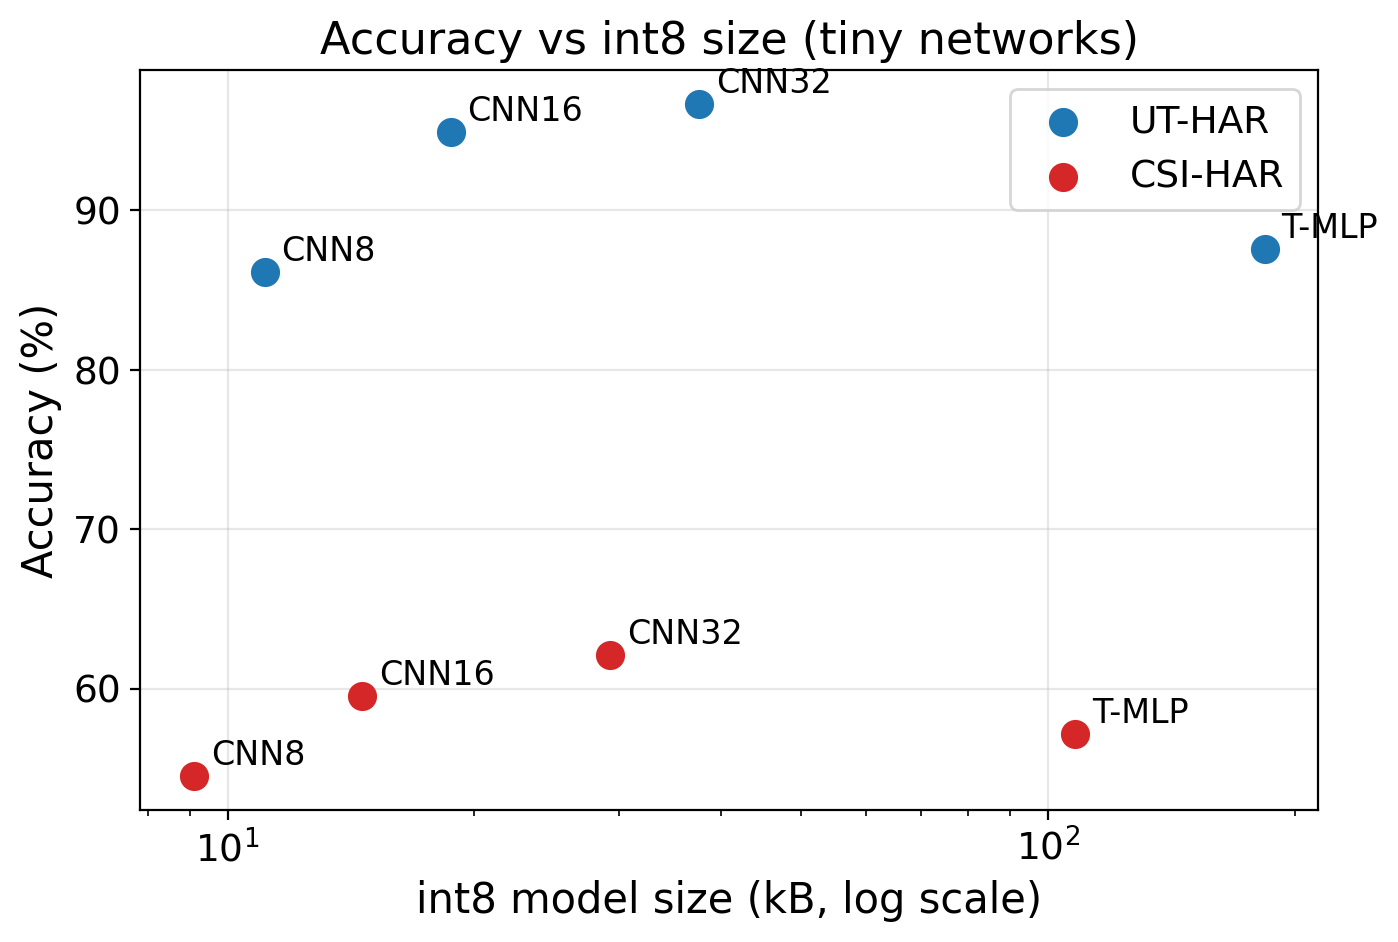
\includegraphics[width=\columnwidth]{fig_frontier.png}
\caption{Accuracy versus int8 size for the tiny networks on both datasets (size on a logarithmic axis). The 16-channel tiny CNN sits at the top-left on both datasets, giving the best accuracy per kilobyte. The int8 file size is a lower bound on on-device cost; the runtime arena, which is what meets the device budget, is measured separately.}
\label{fig:frontier}
\end{figure}

\subsection{ESP32-S3 comparison}
\label{sec:results-s3}
% NEW (measured #9). Flag for Turnitin: prose below is factual, author may reword.
To place the classic ESP32 against a more capable but still commodity board, we flashed the same twelve int8 models to an ESP32-S3 (Xtensa LX7 with the esp-nn SIMD kernels and PSRAM) and measured latency and energy the same way. Table~\ref{tab:s3} reports both boards. The S3 is on average 4.8$\times$ faster and uses about 70\% less energy per inference; the convolutional models gain most (4.6 to 7.8$\times$) because they map onto the vector kernels, while the statistics MLP and the attention-heavy Transformer gain least (1.2 to 1.5$\times$). The classic ESP32 is therefore a conservative reference point for the family: every model that runs on it runs faster and at lower energy on the S3, so our frontier is a conservative reference rather than a strict lower bound on every ESP32-family device or configuration.

\begin{table}[t]
\caption{Measured classic ESP32 versus ESP32-S3 on the same int8 models. Latency and active power are measured on each board; energy is their product. The S3 (LX7 cores with esp-nn SIMD kernels and PSRAM) is on average 4.8$\times$ faster and uses 70\% less energy per inference; the convolutional models benefit most from the vector kernels.}
\label{tab:s3}
\centering
\footnotesize
\setlength{\tabcolsep}{4pt}
\resizebox{\columnwidth}{!}{%
\begin{tabular}{llccccc}
\toprule
Model & Data & Classic (ms) & S3 (ms) & Speedup & Classic (mJ) & S3 (mJ) \\
\midrule
Tiny CNN (8 ch)  & UT  & 14.1  & 2.4   & 5.9$\times$ & 5.0   & 0.66 \\
Flattened MLP   & UT  & 33.3  & 25.3  & 1.3$\times$ & 10.0  & 6.81 \\
Tiny CNN (16 ch) & UT  & 29.7  & 4.1   & 7.2$\times$ & 10.7  & 1.24 \\
Tiny CNN (32 ch) & UT  & 67.8  & 8.7   & 7.7$\times$ & 24.6  & 2.88 \\
Deep CNN         & UT  & 225.6 & 29.1  & 7.8$\times$ & 71.0  & 8.91 \\
Deep Transformer & UT  & 169.8 & 115.5 & 1.5$\times$ & 58.9  & 28.85 \\
Tiny CNN (8 ch)  & CSI & 9.4   & 2.0   & 4.6$\times$ & 3.5   & 0.51 \\
Flattened MLP   & CSI & 19.6  & 14.7  & 1.3$\times$ & 6.0   & 4.16 \\
Tiny CNN (16 ch) & CSI & 20.2  & 3.5   & 5.8$\times$ & 7.7   & 0.98 \\
Tiny CNN (32 ch) & CSI & 46.4  & 6.7   & 6.9$\times$ & 17.5  & 2.18 \\
Deep CNN         & CSI & 243.5 & 40.2  & 6.1$\times$ & 80.7  & 11.86 \\
Deep Transformer & CSI & 320.7 & 266.0 & 1.2$\times$ & 117.8 & 77.04 \\
\bottomrule
\end{tabular}}
\end{table}

\subsection{Live deployment: the full pipeline on-device}
\label{sec:results-live}
% NEW (Major #1, measured 30-min run). Flag for Turnitin: prose is factual, author may reword.
A fielded sensor must run more than isolated inference, so we ran the entire acquisition-to-prediction pipeline on the classic ESP32 in real time (Figure~\ref{fig:live}). The board associates to a 2.4\,GHz access point as a station and pings the gateway so that received packets arrive steadily; the esp-wifi CSI callback delivers per-packet subcarrier data, from which the device forms $T{=}64$ by 52-subcarrier amplitude windows, applies the same per-window normalization as training, int8-quantizes to the deployed input scale, and runs the tiny CNN under TensorFlow Lite Micro. We ran this continuously for 30 minutes; Table~\ref{tab:live} summarizes the result. The pipeline sustained a CSI arrival rate of about 100 packets per second and classified 2{,}825 windows with no dropped windows and no overflow, at a steady 37.6\,ms post-window latency (from the last packet of a window to the label; the capture-to-label time is dominated by the roughly 640\,ms needed to accumulate a 64-packet window at about 100 per second) and an acquisition-bound rate of 1.57 windows per second, while the free internal SRAM varied by only about 2.5\,kB over the whole run and the device never crashed or reset. The full sensing loop, from capture to label, therefore runs and stays stable on the bare PSRAM-less device for the whole run, and not just the isolated inference stage measured elsewhere in this paper. We deliberately do not report a live classification accuracy: the deployed model was trained on a different-domain public CSI corpus rather than on this radio and room, so an over-the-air accuracy number would measure domain shift, not the pipeline; in-domain data collection and retraining on the target device is the natural next step (Section~\ref{sec:discussion}).

\begin{table}[t]
\caption{Live deployment on the classic ESP32: the full capture-to-label pipeline run continuously for 30 minutes (2.4\,GHz station, CSI from received packets, 16-channel tiny CNN). ``Post-window latency'' is the time from the last packet of a completed 64-packet window to the emitted label (preprocessing plus inference); it is not the capture-to-label time, which is dominated by the roughly 640\,ms needed to accumulate 64 packets at about 100 per second. The live window rate (1.57/s) is therefore bounded by non-overlapping window acquisition, not by inference, whose isolated rate is far higher (Section~\ref{sec:discussion}). ``Packet / window loss'' is measured at the CSI callback (buffer level): no delivered callback was dropped and no window overflowed in this run; upstream 802.11 losses before the callback are not observable here. Classification accuracy is not reported (the model was trained on a different-domain public dataset, so a live number would measure domain shift).}
\label{tab:live}
\centering
\footnotesize
\begin{tabular}{lr}
\toprule
Metric & Value \\
\midrule
Run duration                  & 30 min \\
CSI packets received          & 180{,}815 \\
Packet arrival rate           & 100.5 /s \\
Packet / window loss (buffer) & 0.00\% (0 dropped) \\
Windows classified            & 2{,}825 \\
Post-window latency (last pkt$\to$label) & 37.6 ms (35.9--37.7) \\
Live window rate (acquisition-bound) & 1.57 windows/s \\
Free internal SRAM            & 134.6--137.1 kB (2.5 kB jitter) \\
Largest free block            & 88.0--92.0 kB \\
Crashes / watchdog resets     & 0 \\
\bottomrule
\end{tabular}
\end{table}

% R2-11c: enlarged to a two-column figure (reviewer: Figure 7 is very small).
\begin{figure*}[tbp]
\centering
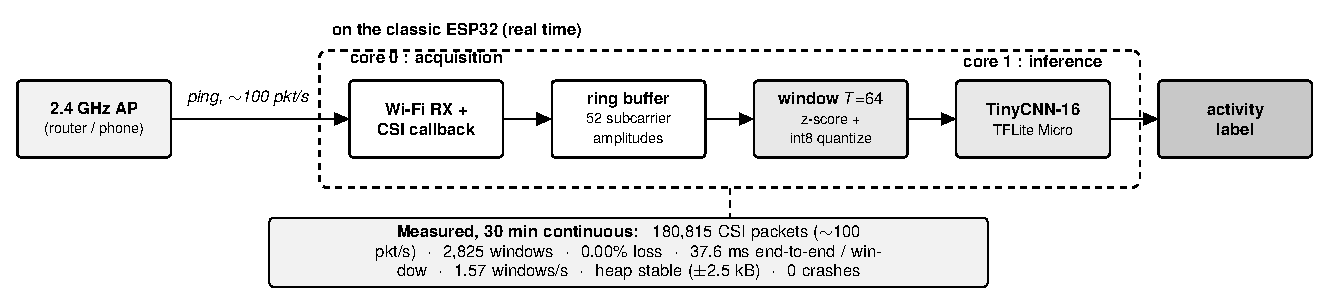
\includegraphics[width=0.86\textwidth]{fig_live_pipeline.pdf}
\caption{Live on-device WiFi-CSI pipeline on the classic ESP32: over-the-air CSI capture, windowing and per-window normalization, int8 quantization, and TensorFlow Lite Micro inference, all running on the device in real time.}
\label{fig:live}
\end{figure*}

\subsection{Per-class behaviour and statistical analysis}
\label{sec:results-perclass}
Accuracy alone can hide class-dependent behaviour, so for the subject-independent CSI-HAR setting we pool the leave-one-user-out predictions across the three folds, so that every sample is predicted exactly once as an unseen user, and report macro precision, recall, and F1 for a tiny CNN, a Random Forest, and a deep CNN in Table~\ref{tab:prf}. The three models track their accuracy closely, with macro F1 within about a point of accuracy in every case, so no model is inflating its accuracy by collapsing onto a majority class. Figure~\ref{fig:cm} shows the corresponding confusion matrices, and their structure is consistent across models and physically sensible. The largest single error is between the two locomotion activities: most run windows are classified as walk (41 of 60 for the tiny CNN, 34 of 60 for the deep CNN), because on a single link the two produce similar broadband amplitude variation and differ mainly in speed, which quantized amplitude features capture only weakly. Fall is the hardest class, with the lowest recall of any activity (about 38\%): its windows scatter into bend, stand up, and run, consistent with a fall being a brief transient whose onset resembles the start of several other motions. Among the low-motion postures, lie down and sit down are mutually confused (11 lie-down windows read as sit down), as both are near-static end states with little dynamic signature. What matters for the argument of this paper is that the same activity pairs dominate the confusion matrices of both the tiny model and the five-times-larger deep model, which is consistent with a representation limitation of single-link amplitude CSI rather than a shortage of model capacity (we did not run a representation ablation, so we do not claim to isolate representation from capacity). A per-window paired analysis supports this at the sample level without overstating it: the tiny CNN and the deep CNN agree on 71\% of the pooled leave-one-user-out windows, and 51\% of the tiny model's errors are also errors of the deep model. So the two models make substantially, though not identically, the same mistakes; the shared-error rate is well above chance but the models are not error-equivalent, which is what the aggregate matrices alone could not establish.

\begin{table}[t]
\caption{Macro precision, recall, and F1 on CSI-HAR under subject-independent leave-one-user-out, with predictions pooled across the three folds. Macro F1 stays within about a point of accuracy for all three models, so accuracy is not driven by a majority-class bias. Because the accuracy here is computed from predictions pooled across folds rather than averaged over per-fold accuracies, it differs by one to two points from the fold-averaged deep-CNN value in Table~\ref{tab:deep}; both are within the cross-subject fold variance.}
\label{tab:prf}
\centering
\footnotesize
\setlength{\tabcolsep}{4pt}
\resizebox{\columnwidth}{!}{%
\begin{tabular}{lcccc}
\toprule
Model & Accuracy (\%) & Precision (\%) & Recall (\%) & F1 (\%) \\
\midrule
Tiny CNN (32 ch) & 62.14 & 62.03 & 62.14 & 60.94 \\
Random Forest    & 57.38 & 58.55 & 57.38 & 56.53 \\
Deep CNN         & 66.19 & 66.21 & 66.19 & 65.51 \\
\bottomrule
\end{tabular}}
\end{table}

\begin{figure*}[!t]
\centering
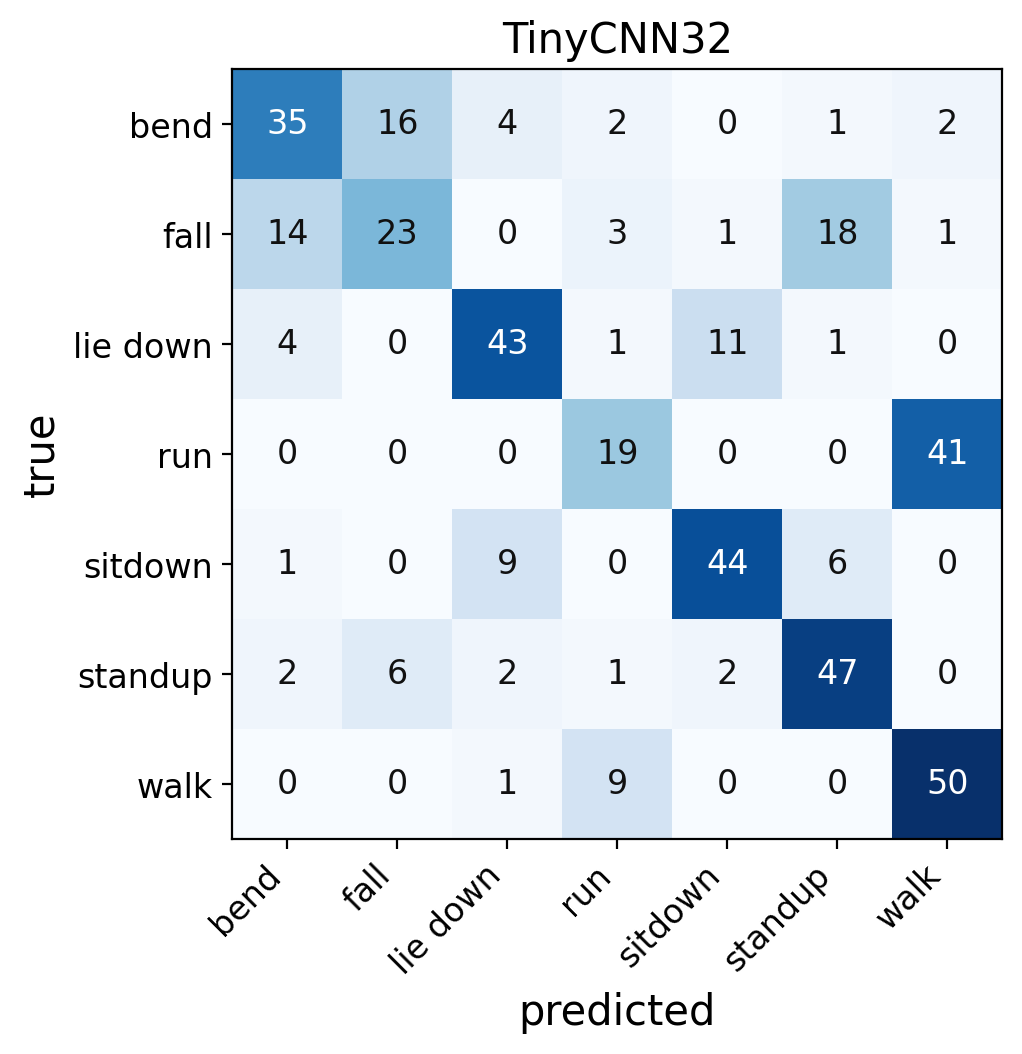
\includegraphics[width=0.32\textwidth]{fig_cm_TinyCNN32.png}\hfill
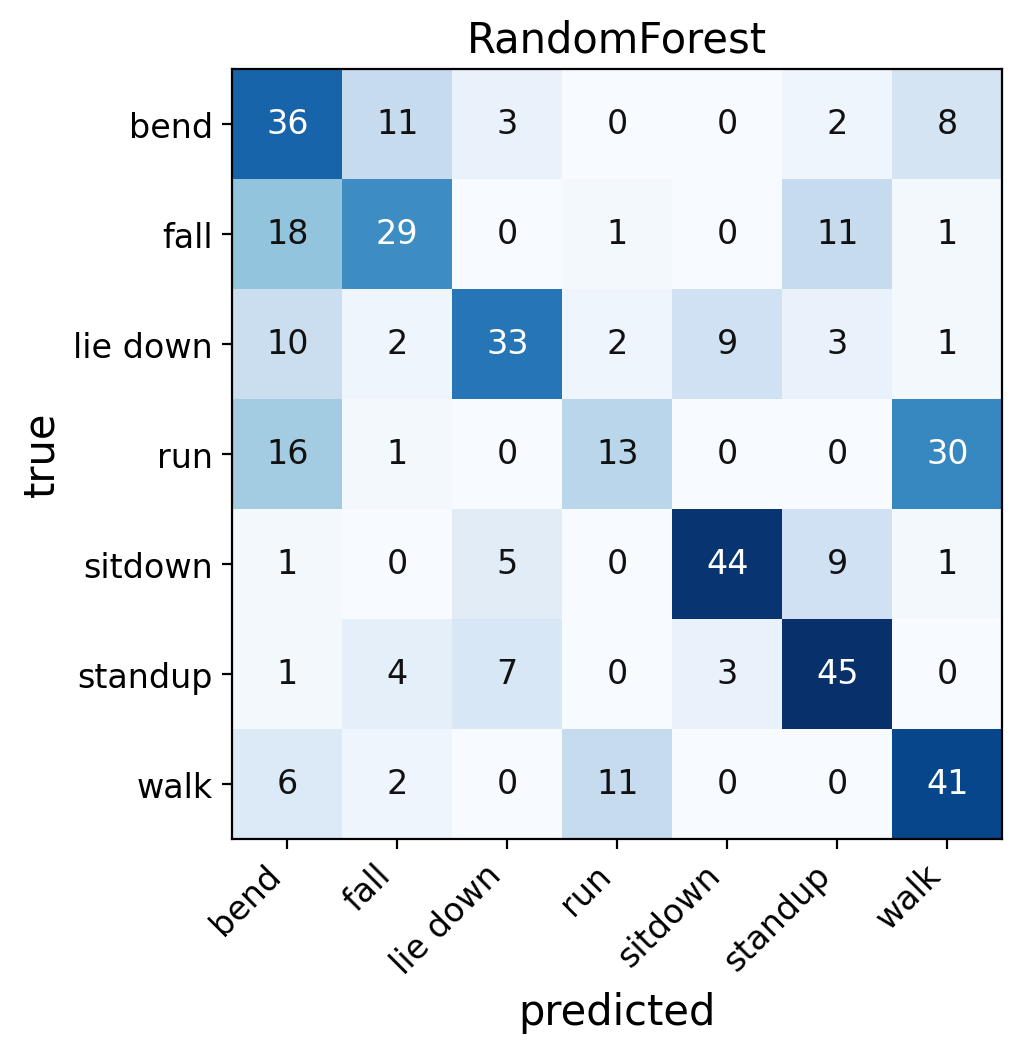
\includegraphics[width=0.32\textwidth]{fig_cm_RandomForest.png}\hfill
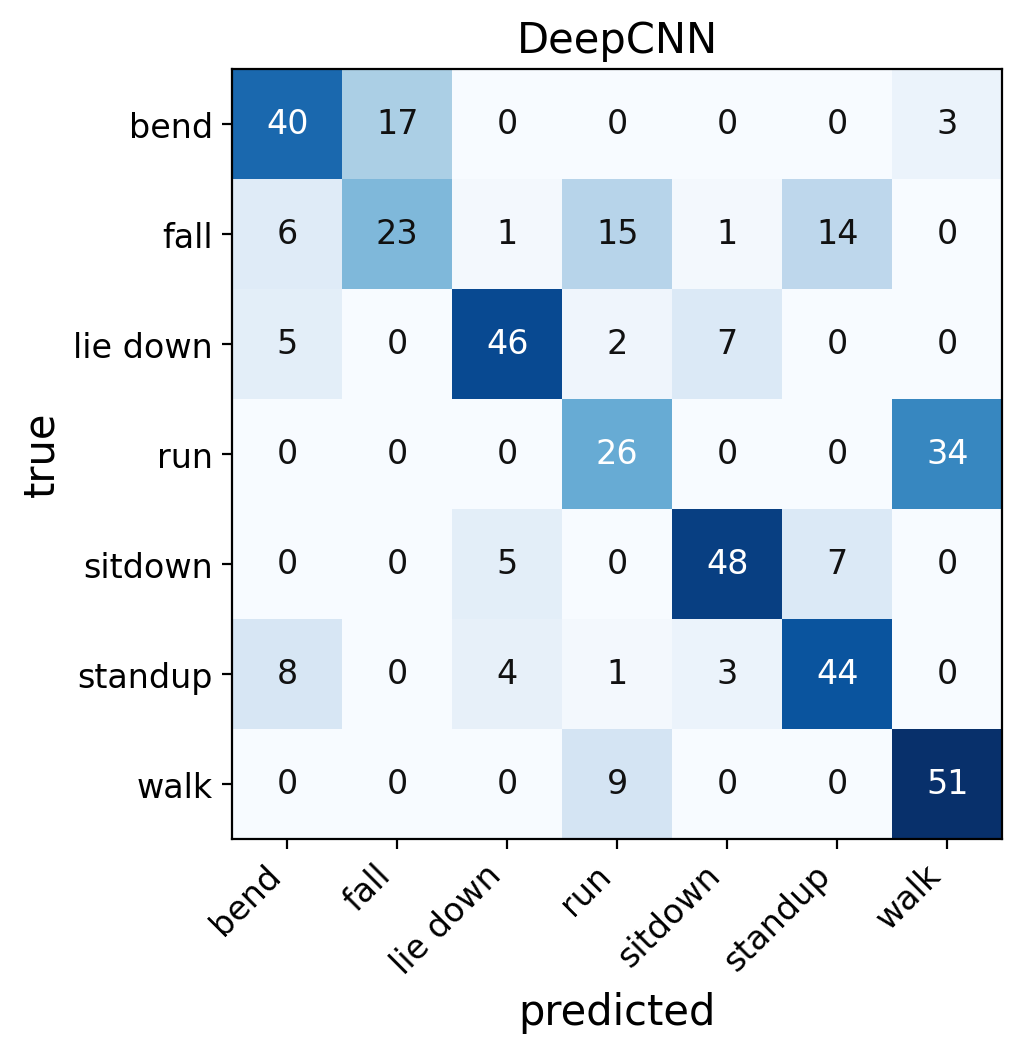
\includegraphics[width=0.32\textwidth]{fig_cm_DeepCNN.png}
\caption{Confusion matrices on CSI-HAR under subject-independent leave-one-user-out (predictions pooled across the three folds) for the tiny CNN, the Random Forest, and the deep CNN. The dominant error is run misread as walk; fall has the lowest recall and scatters into bend, stand up, and run; and the near-static lie down and sit down are mutually confused. The same errors persist from the tiny model to the deep one.}
\label{fig:cm}
\end{figure*}

Because the dataset has only three users, the most informative summary is per-user rather than a single pooled number. Table~\ref{tab:peruser} reports leave-one-user-out accuracy for each held-out user, with the neural models averaged over three seeds so the stochastic-training variance is visible. The picture is heterogeneous: the tiny and 32-channel CNNs and the Random Forest are within a few points of each other on users 1 and 2, but user 3 is both the hardest and the most seed-sensitive (the 16-channel CNN ranges $\pm$8 points across seeds), which is exactly the kind of small-sample instability that a single averaged number hides. This per-user, multi-seed view is the primary evidence for the model comparison; we report the aggregate significance tests below only for completeness.

\begin{table}[t]
\caption{Per-held-out-user leave-one-user-out accuracy (\%) on CSI-HAR, neural models averaged over three seeds (mean $\pm$ std). These values are from the dedicated multi-seed metrics run; averaging the three folds gives a leave-one-user-out mean that differs by one to two points from the frontier-run entry in Table~\ref{tab:frontier} (a different seed set), both within the fold-to-fold variance. With only three users the per-user spread and the seed sensitivity, especially on user 3, are more informative than a single pooled accuracy or a significance test.}
\label{tab:peruser}
\centering
\footnotesize
\setlength{\tabcolsep}{4pt}
\resizebox{\columnwidth}{!}{%
\begin{tabular}{lccc}
\toprule
Held-out user & TinyCNN-16 & TinyCNN-32 & Rand. Forest \\
\midrule
User 1 & 59.05 $\pm$ 1.35 & 59.05 $\pm$ 1.47 & 59.29 \\
User 2 & 57.86 $\pm$ 3.09 & 59.05 $\pm$ 3.32 & 60.00 \\
User 3 & 55.48 $\pm$ 8.19 & 66.67 $\pm$ 1.21 & 52.86 \\
\bottomrule
\end{tabular}}
\end{table}

We also asked whether the model differences are statistically meaningful. With only three held-out users the power is very low, so we treat these tests as exploratory: a Friedman test across the tiny CNN, deep CNN, Transformer, and Random Forest over the three folds is not significant ($\chi^2 = 4.44$, $p = 0.22$), and a Wilcoxon signed-rank test between the deep CNN and the Transformer likewise ($p = 0.25$). With $n=3$ these cannot establish a difference or an equivalence and are reported only for completeness; what we rely on instead is the consistent effect size (across every fold the tiny model stays within a few points of the deep models). A properly powered comparison would need a many-subject corpus, which we flag as future work.

\subsection{The generalization gap: an exploratory case study}
\label{sec:results-gap}
The deployment results show that fitting a model on the device is largely solved. The harder question is whether a model works on a person it was not trained on. To isolate this, we evaluated the same models, features, and training pipeline on CSI-HAR under two protocols that differ only in how the data is split: a random stratified 80/20 split, in which recordings from every user appear in both train and test, and the subject-independent leave-one-user-out protocol used throughout this paper. Table~\ref{tab:gengap} and Figure~\ref{fig:gengap} report both.

The gap is large and consistent. Every model loses 25 to 33 percentage points when the test user is unseen, a mean drop of 29 points (the seven-class chance level is 14.3\%, so the leave-one-user-out accuracies remain well above chance). The 32-channel tiny CNN reads 96.4\% on the random split, which is in the range CSI-HAR papers commonly report, but only 63.1\% leave-one-user-out; the Random Forest falls from 83.1\% to 58.1\%. Because nothing changes between the two columns except the split, the gap is not a property of any model or of its size. It is the cost of generalizing across people, and a random split hides it by letting the model memorize each user's channel signature. This is why we report subject-independent accuracy throughout. On this three-user dataset the harder problem is generalization rather than deployment; we offer this as an exploratory case-study observation rather than a universal law, since the chip runs every model but the cross-subject evidence here rests on only three users.

\begin{table}[t]
\caption{Cross-subject generalization gap on CSI-HAR. Identical models, features, and training; the only difference is the split. ``Random'' is a stratified 80/20 split over three seeds, in which each user appears in both train and test; ``LOUO'' is subject-independent leave-one-user-out over the three users. The gap is the accuracy lost when the test person is unseen. These values come from the dedicated generalization-gap run and differ by about a point from the corresponding entries in Table~\ref{tab:frontier} owing to different random seeds; both lie within the fold-to-fold variance.}
\label{tab:gengap}
\centering
\footnotesize
\begin{tabular}{lccc}
\toprule
Model & Random split (\%) & LOUO (\%) & Gap (pts) \\
\midrule
Decision Tree    & 69.4 & 40.6 & 28.9 \\
Random Forest    & 83.1 & 58.1 & 25.0 \\
MLP (statistics) & 85.2 & 56.9 & 28.3 \\
Tiny CNN (16 ch) & 92.1 & 62.1 & 29.9 \\
Tiny CNN (32 ch) & 96.4 & 63.1 & 33.3 \\
Flattened MLP   & 87.7 & 56.9 & 30.8 \\
\midrule
Mean             & 85.7 & 56.3 & \textbf{29.4} \\
\bottomrule
\end{tabular}
\end{table}

\begin{figure}[tbp]
\centering
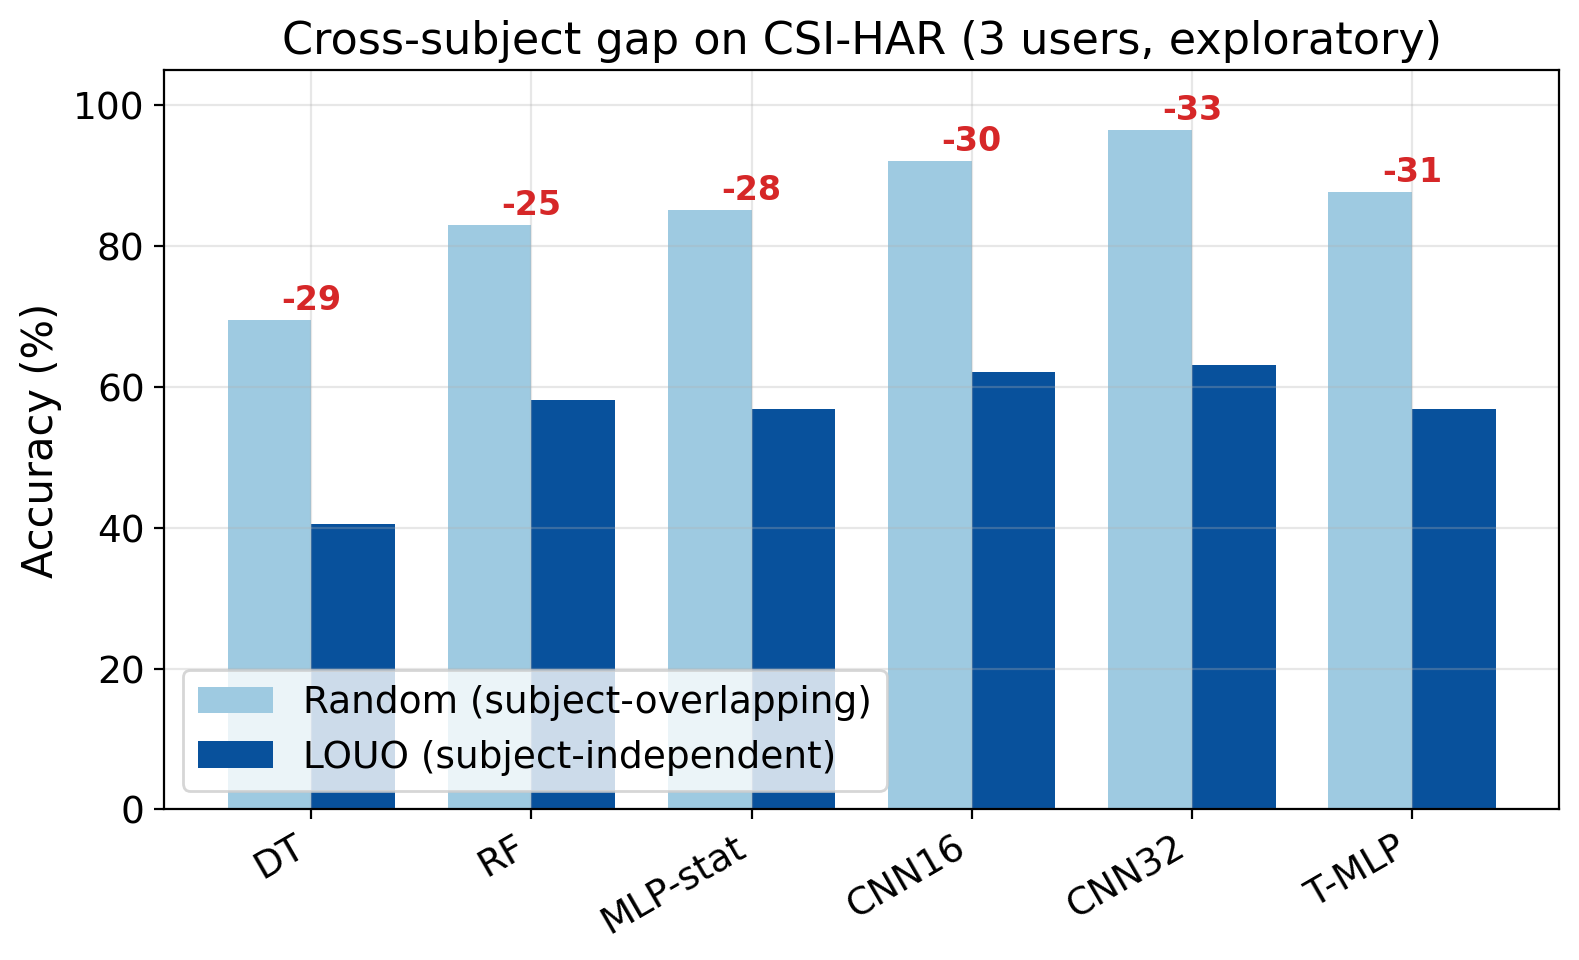
\includegraphics[width=\columnwidth]{fig_gengap.png}
\caption{The cross-subject generalization gap on CSI-HAR. The same models score much higher on a random split (light bars) than under subject-independent leave-one-user-out (dark bars); the red number is the accuracy lost per model. The mean drop of 29 points is the cost of recognizing an unseen person, and it is invisible to a random split.}
\label{fig:gengap}
\end{figure}

To check that this gap is not an artefact of the three-user CSI-HAR set, we reproduced the same random-versus-subject-independent contrast on a much larger public WiFi-CSI corpus, CSI-Bench~\cite{csibench2025}, a four-class task on 35 users (Table~\ref{tab:gengap-ext}, Figure~\ref{fig:gengap-ext}). We ran two classifiers there: the deployed tiny CNN and, as a light off-device reference, a Random Forest on per-subcarrier amplitude statistics. The deployed tiny CNN falls from 93.3\% on a random split to 62.6\% under a subject-independent split, a 30.8-point drop, and the Random Forest from 84.1\% to 51.7\% (32.4 points); both remain well above the 25\% chance level. The gap therefore holds on a many-user dataset for the actual deployed architecture, not only for a proxy, and is not specific to the small three-user set. It is measured off-device on a different four-class task, so it establishes the breadth of the cross-subject phenomenon rather than the on-device deployability result, which rests on CSI-HAR; a fully powered on-hardware cross-subject study on a many-subject, multi-room corpus remains the most important extension.

\begin{table}[t]
\caption{Cross-subject generalization gap across datasets and classifiers. Moving from a random (subject-overlapping) split to a subject-independent split lowers accuracy by about 30 points in every case, and the subject-independent accuracy stays well above chance throughout, so the effect is a genuine graded gap rather than a floor effect and is not specific to the small three-user set. On the 35-user CSI-Bench corpus the gap holds for the deployed tiny CNN (30.8 points), not only for the light off-device Random Forest reference (32.4 points).}
\label{tab:gengap-ext}
\centering
\footnotesize
\setlength{\tabcolsep}{3.5pt}
\resizebox{\columnwidth}{!}{%
\begin{tabular}{llcccc}
\toprule
Dataset (subjects) & Model & Random (\%) & Subject-indep. (\%) & Chance (\%) & Drop \\
\midrule
CSI-HAR (3)    & Tiny CNN & 92.1 & 62.1 & 14.3 & 30.0 pts \\
CSI-Bench (35) & Tiny CNN & 93.3 & 62.6 & 25.0 & 30.8 pts \\
CSI-Bench (35) & Rand.\ Forest & 84.1 & 51.7 & 25.0 & 32.4 pts \\
\bottomrule
\end{tabular}}
\end{table}

\begin{figure}[tbp]
\centering
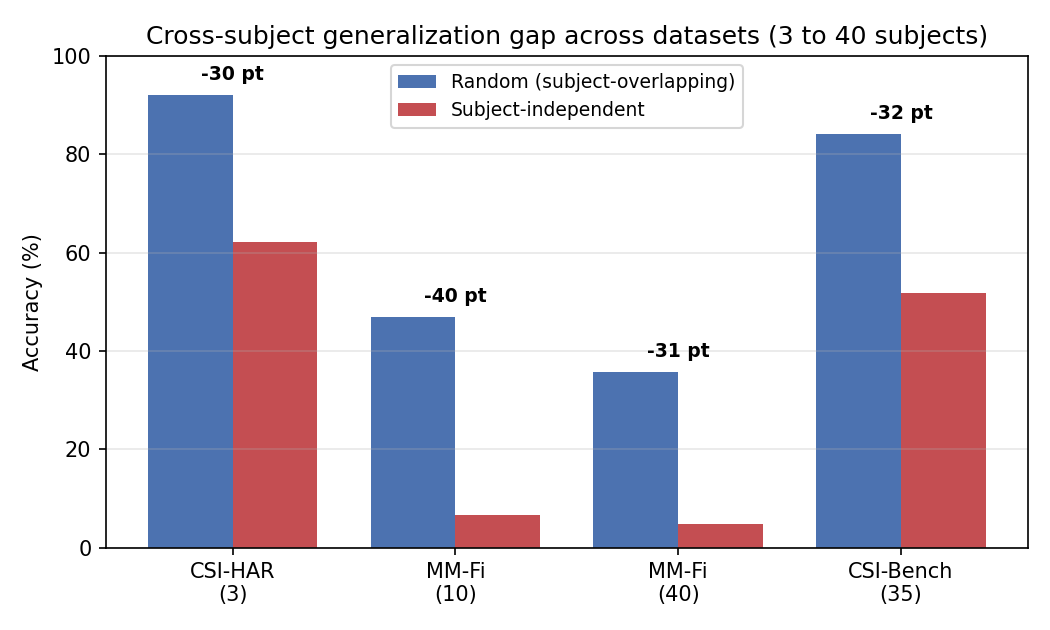
\includegraphics[width=\columnwidth]{fig_gengap_external.png}
\caption{The cross-subject generalization gap reproduces on a many-user dataset and for the deployed architecture: on CSI-HAR (3 users) and on CSI-Bench (35 users) the tiny CNN drops by about 30 points from a random split to a subject-independent split, and the light Random Forest reference on CSI-Bench drops similarly, all staying above chance (dashed lines).}
\label{fig:gengap-ext}
\end{figure}

Because the gap is a cross-subject effect rather than a capacity limit, the natural remedy is to give the model a small amount of data from the target person rather than a larger model. We tested this directly with a personalization sweep: for each held-out user we add $k$ calibration windows from that user (counted as a total across the seven activities, not per class, and drawn at random from the user's recordings) to the training set, retrain, and test on the user's remaining windows, averaging over the three users and three seeds. Figure~\ref{fig:personalization} shows the result. At $k=0$ this reproduces the zero-shot leave-one-user-out accuracy (61.9\% for the tiny CNN, 58.1\% for the Random Forest); adding only ten calibration samples raises the tiny CNN to 71.0\%, and forty samples raise it to 87.0\%, a recovery of roughly 25 points from a small number of labelled samples from the target user. The Random Forest improves more slowly, to 74.7\% at $k=40$. This supports the reading that the deployed fix is a short per-user calibration rather than a bigger network, which the device can well afford given microsecond-scale classical inference and tens-of-milliseconds neural inference. With only three users this is a demonstration of the effect rather than a large-scale study, but the direction is clear and consistent across both model families.

\begin{figure}[tbp]
\centering
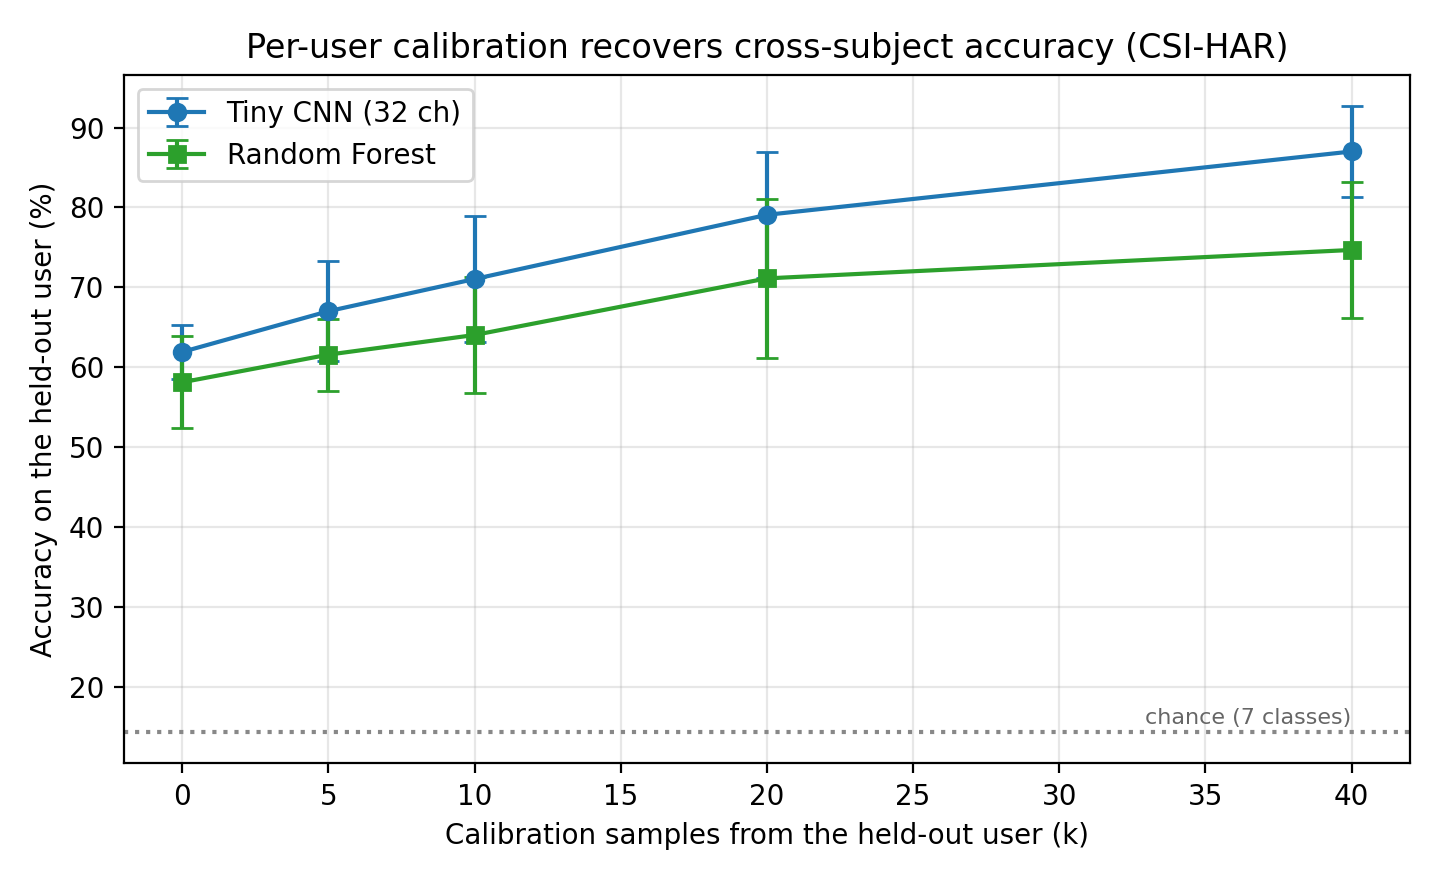
\includegraphics[width=\columnwidth]{fig_personalization.png}
\caption{Per-user calibration recovers cross-subject accuracy on CSI-HAR. For each held-out user, $k$ calibration windows from that user (total across the seven activities, not per class) are added to training and accuracy is measured on the user's remaining windows (mean over three users and three seeds). $k=0$ is the zero-shot leave-one-user-out point; adding ten to forty samples recovers much of the cross-subject gap, more sharply for the tiny CNN than for the Random Forest.}
\label{fig:personalization}
\end{figure}

\section{Discussion}
\label{sec:discussion}

\subsection{What runs and what blocks on a bare ESP32}
The frontier answers the title question more permissively than the chip's reputation suggests. On the PSRAM-less classic ESP32 the deployable options for WiFi CSI HAR include the classical learners, the tiny CNNs, and a deep CNN and convolution-augmented Transformer, all of which allocate and run within tens of kilobytes. What the small models offer is efficiency, not exclusivity: on the saturated UT-HAR benchmark a statistics MLP reaches 95.3\% and the 32-channel tiny CNN 96.7\% (a 37.6\,kB int8 model), within a point or two of the deep models at a fraction of the size and latency, so a practitioner should start with the tiny and classical tiers and reach for a deep CNN or Transformer only if accuracy demands it. The barriers that remain are narrower than a blanket memory limit. Convertibility is the hard gate: recurrent and state-space models do not reach the runtime at all without custom operators, because their fused recurrent and dynamic-tensor operators are outside the builtin set; the Chebyshev-KAN converts but fails to allocate as exported by the default converter, an operator-mapping limitation rather than a memory ceiling, since the much larger CNN and Transformer allocate comfortably on the same device. We initially assumed a memory wall blocked all deep models, and flashing them to the board showed that assumption was wrong, which is the value of bare-device characterization over a GPU-only or PSRAM-equipped comparison, and it also explains why prior on-device CSI work, navigating the same conversion limits, tends to favour convolutional models.

\subsection{Generalization is the binding constraint}
The two halves of the study point in the same direction: once the deep CNN and Transformer are shown to run on the bare board, compute and memory are no longer what limits CSI HAR on this hardware, while the leave-one-user-out results show a mean 29-point drop when the test person is unseen (Section~\ref{sec:results-gap}). A plausible explanation, consistent with this limited evidence, is physical rather than statistical: CSI amplitude encodes the multipath channel, which is shaped by the person's body geometry and gait and by their position relative to the link, so an unseen person is an out-of-distribution input whose channel signature the model has not learned. This is why increasing capacity did not help (the larger Transformer was no more robust across people than the tiny CNN) while a few calibration samples did: adding only forty labelled samples from the target user lifts the tiny CNN from 62\% to 87\% on that user (Figure~\ref{fig:personalization}). The practical consequence is that effort is better spent on generalization than on shrinking the model, and that subject-independent accuracy should be reported as standard practice, because a random split on a small multi-user corpus reports a number the deployed device will not reach (a practitioner who reads 96\% will see about 63\% on a new user). Cross-subject methods such as domain adaptation, which would reduce even the calibration cost, are the substantive open problem. This also reinforces why the smallest models are attractive for the most constrained hardware: the classical learners are one to three orders of magnitude smaller than the networks, run in microseconds atop a shared 1 to 2\,ms feature-extraction step, and stay competitive on the saturated benchmark, so for a sensing task that must share a microcontroller with an application their predictability and small footprint are decisive.

\subsection{Practical deployment under a live radio}
A fielded sensor runs a four-stage real-time pipeline (Figure~\ref{fig:pipeline}), which we built and ran live on the classic ESP32 (Section~\ref{sec:results-live}). Two practical considerations follow. First, timing is comfortable: a tiny CNN classifies a window in tens of milliseconds, well above the rate at which non-overlapping activity windows arrive, and even the deep models (an isolated 3 to 6 windows per second) remain adequate for activity-scale events. Second, sensing and inference must share the chip. The ESP32 is dual-core, so acquisition can run on one core while inference runs on the other, but an active WiFi stack claims internal SRAM: initializing the radio in station mode drops the largest free internal block from 152\,kB to 108\,kB, and in the live run it is about 88 to 92\,kB once the application and CSI ring buffer are resident. Every deployable model still fits and runs under this reduced budget, with latencies within a millisecond of the radio-off figures (Supplementary Material, Table~S7). System-level headroom, not the arena, is the real constraint: after a 54\,kB Transformer arena the live budget leaves only about 36\,kB for application code and network buffers, so the ``no memory wall'' conclusion holds for fitting the model but the deep models leave little room for a concurrent networking application, whereas the tiny and classical tiers leave ample margin. Runtime stability is confirmed by the 30-minute live run (Section~\ref{sec:results-live}): the static tensor arena performs no per-inference dynamic allocation, so it cannot leak or fragment, and the latency did not drift and no window was lost, though multi-hour operation and thermal drift remain untested.

\subsection{Limitations}
We group the limitations into three kinds so that the scope of the claims is unambiguous.

\emph{Dataset size and diversity.} The generalization results rest on CSI-HAR, which has only three users, so the leave-one-user-out evaluation runs over three folds and the cross-subject numbers, while consistent, are a demonstration of the effect rather than a large-scale study; the three-user size is also why we treat the significance tests as exploratory (Section~\ref{sec:results-perclass}). UT-HAR is larger but saturated and not subject-partitioned, so it cannot show the gap. We add NTU-Fi\_HAR as a third dataset for the frontier (Section~\ref{sec:results-frontier}), which confirms the accuracy-versus-cost ordering but is itself saturated and single-session. To test the cross-subject gap on more than three users we reproduced it on a larger public corpus, CSI-Bench (35 users), where both the deployed tiny CNN (30.8 points) and a light Random Forest reference (32.4 points) show the same graded drop that stays above chance (Section~\ref{sec:results-gap}, Table~\ref{tab:gengap-ext}). That check is off-device and on a different four-class task, so a fully powered on-hardware cross-subject study on a many-subject, multi-room corpus remains the most important extension.

\emph{Hardware constraints.} All device measurements come from a single classic ESP32 board. Energy is measured on that board with an INA219 current sensor (Section~\ref{sec:results-ondevice}); any datasheet-derived figure we quote for context is presented as an estimate over the full 30 to 68\,mA range and not as a single value or bound. We also run the same int8 models on an ESP32-S3 (which adds PSRAM and the esp-nn vector kernels): it is on average 4.8$\times$ faster and uses about 70\% less energy per inference than the classic ESP32, with the convolutional models benefiting most from the SIMD kernels (Section~\ref{sec:results-s3}, Table~\ref{tab:s3}). The classic ESP32 therefore characterizes the weakest and most constrained commodity target, and the S3 figures bound the speedup available on the more capable board rather than being left to speculation. For context, Armenta-Garcia \emph{et~al.}~\cite{hernandez2025tools} report 232\,ms per inference and a 127\,kB footprint (using external PSRAM) for a quantized DenseNet CSI model on the ESP32-S3, whereas our feed-forward deep models run in 170 to 321\,ms on the PSRAM-less classic ESP32 through the export pipeline described here.

\emph{Deployment assumptions.} On-device latency, throughput, and memory are measured for isolated inference with the WiFi and Bluetooth stacks disabled, which is the clean characterization condition but not a live capture. A deployed sensor must acquire CSI concurrently with inference and with the radio active, which reduces the free internal block and adds duty-cycle pressure (Section~\ref{sec:discussion}); we do build and validate a 30-minute live-capture pipeline (Section~\ref{sec:results-live}), but we do not evaluate its in-domain classification accuracy, and multi-hour and multi-day operation, thermal drift, and upstream packet loss remain untested. The live experiment therefore establishes on-device system throughput, buffering, and runtime stability under real WiFi traffic, not live recognition accuracy. The deep-tier UT-HAR accuracies come from the companion single-pipeline benchmark, whereas the CSI-HAR numbers and all on-device outcomes are measured directly by flashing each model.

%\section{Conclusion}
%\label{sec:conclusion}
%In this paper, we presented a deployability frontier for WiFi CSI human activity recognition on the cheapest and most constrained commodity WiFi microcontroller, the PSRAM-less classic ESP32. Across two datasets and a graded set of models from classical learners through tiny networks to five deep architectures, we showed by flashing each to the board that the recurrent and state-space models do not convert to the microcontroller runtime and the Kolmogorov-Arnold model fails to allocate, but that a full deep CNN and a Transformer do run on the bare classic ESP32, alongside the tiny and classical models. There is no general memory wall for feed-forward CSI models on this device. On the saturated UT-HAR benchmark the small models are competitive (a tiny CNN at 96.7\% and a classical multilayer perceptron at 95.3\%) at a fraction of the cost, while a subject-independent evaluation on CSI-HAR exposes the binding constraint: the same models drop by a mean of 29 percentage points (the best from 96\% to 63\%) when the test person is unseen, so our experiments suggest that cross-subject generalization may be a more significant challenge than memory limitations at this scale. We measured on the physical device (at 240\,MHz) that the tiny networks allocate with an 8 to 13\,kB arena and run in 9 to 68\,ms per inference, and that the deep CNN and Transformer allocate within 10 to 54\,kB and run in 170 to 321\,ms. The contribution is a practitioner-oriented, reproducible map of what is deployable on the bare device, with all code, models, and measurement firmware released. Future work includes a precise on-device energy study with a current probe, extending the frontier to additional microcontrollers, datasets, and live-capture validation, and testing whether the recurrent, state-space, and Kolmogorov-Arnold conversion and allocation failures are specific to TensorFlow Lite for Microcontrollers by porting the same models through other embedded runtimes such as microTVM, Apache TVM, or Edge Impulse.

\section{Conclusion}
In this paper, we established a comprehensive deployability frontier for WiFi CSI-based human activity recognition on the most resource-constrained commodity WiFi microcontroller: the classic, PSRAM-less ESP32. By flashing a wide spectrum of models to physical hardware operating at 240 MHz, we proved that deep feed-forward architectures, including full deep CNNs and convolution-augmented Transformers, can execute on the bare chip within a 10 to 54 KB tensor arena and an inference latency of 170 to 321 ms. Meanwhile, lightweight models such as tiny CNNs run in just 9 to 68 ms using an 8 to 13 KB arena. These findings correct a widespread assumption in the community by demonstrating that on-device feed-forward CSI inference is not blocked by a chip-level memory wall.
Instead, deployment friction stems from two distinct factors. On the software side, recurrent, state-space, and Kolmogorov-Arnold architectures fail due to runtime conversion and memory allocation limits within TensorFlow Lite for Microcontrollers (TFLM). On the algorithmic side, subject-independent Leave-One-User-Out (LOUO) evaluations expose severe performance degradation, with accuracy dropping by an average of 29 percentage points (and from 96\% down to 63\% for the best model) on unseen individuals. This confirms that cross-subject generalization presents a far more critical bottleneck than on-chip memory limits for real-world CSI HAR deployment.
Beyond the deployability frontier, we characterized the classic ESP32 in depth on real hardware: per-inference energy measured directly with an INA219 current sensor, a head-to-head comparison against the PSRAM-equipped ESP32-S3, and a 30-minute live capture-to-label pipeline that sustained real WiFi traffic with no window loss or memory drift. To support reproducible edge AI research, all code, trained model artifacts, and measurement firmware have been open-sourced. Future work will focus on higher-bandwidth energy profiling and multi-board characterization, expanding the deployability map to additional microcontroller architectures, and live-capture field validation that reports in-domain recognition accuracy. Furthermore, we plan to port the failed recurrent, state-space, and Kolmogorov-Arnold models through alternative embedded runtimes, such as microTVM, Apache TVM, and Edge Impulse, to determine whether these deployment failures are intrinsic to the architectures or artifacts of TFLM operator support.

\section*{Data and Code Availability}
All source code, the ESP32 and ESP32-S3 measurement firmware, the trained and int8-quantized models, the emlearn C exports, and the raw measurement logs and scripts that regenerate the tables and figures are released at \url{https://github.com/ahmadshahbazzz/esp32-csi-har-frontier}. A versioned Zenodo archive with a citable DOI will be minted from the tagged release at acceptance. The public CSI datasets are obtained from their original authors as cited and are not redistributed here.

\begin{thebibliography}{99}

\bibitem{halperin2011csi}
D. Halperin, W. Hu, A. Sheth, and D. Wetherall, ``Tool release: gathering 802.11n traces with channel state information,'' \emph{ACM SIGCOMM Comput. Commun. Rev.}, vol. 41, no. 1, p. 53, Jan. 2011, doi: 10.1145/1925861.1925870.

\bibitem{ma2019wifi}
Y. Ma, G. Zhou, and S. Wang, ``WiFi sensing with channel state information: a survey,'' \emph{ACM Comput. Surv.}, vol. 52, no. 3, pp. 1--36, Jun. 2019, doi: 10.1145/3310194.

\bibitem{yang2023sensefi}
J. Yang, X. Chen, H. Zou, D. Wang, Q. Xu, and L. Xie, ``SenseFi: a library and benchmark on deep-learning-empowered WiFi human sensing,'' \emph{Patterns}, vol. 4, no. 3, p. 100703, Mar. 2023, doi: 10.1016/j.patter.2023.100703.

\bibitem{hernandez2025tools}
J. A. Armenta-Garcia, F. F. Gonzalez-Navarro, J. Caro-Gutierrez, and C. I. Garcia-Reyes, ``Tools and methods for achieving Wi-Fi sensing in embedded devices,'' \emph{Sensors}, vol. 25, no. 19, p. 6220, Oct. 2025, doi: 10.3390/s25196220.

\bibitem{espfihar2026}
Z. Wen, Y. Ruan, X. Wang, and J. Zhou, ``ESP-Fi HAR: a low-power WiFi CSI dataset for ad-hoc IoT human activity recognition,'' \emph{Ad Hoc Netw.}, vol. 186, art. 104192, 2026, doi: 10.1016/j.adhoc.2026.104192.

\bibitem{chen2019ablstm}
Z. Chen, L. Zhang, C. Jiang, Z. Cao, and W. Cui, ``WiFi CSI based passive human activity recognition using attention based BLSTM,'' \emph{IEEE Trans. Mobile Comput.}, vol. 18, no. 11, pp. 2714--2724, Nov. 2019, doi: 10.1109/TMC.2018.2878233.

\bibitem{li2021that}
B. Li, W. Cui, W. Wang, L. Zhang, Z. Chen, and M. Wu, ``Two-stream convolution augmented transformer for human activity recognition,'' in \emph{Proc. AAAI Conf. Artif. Intell.}, vol. 35, no. 1, 2021, pp. 286--293, doi: 10.1609/aaai.v35i1.16103.

\bibitem{khan2025lightweight}
H. Kang, D. Kim, and K.-A. Toh, ``Human activity recognition through augmented WiFi CSI signals by lightweight attention-GRU,'' \emph{Sensors}, vol. 25, no. 5, p. 1547, Mar. 2025, doi: 10.3390/s25051547.

\bibitem{pacsi2025}
T. D. Quy, C.-Y. Lin, and T. K. Shih, ``Enhanced human activity recognition using Wi-Fi sensing: leveraging phase and amplitude with attention mechanisms,'' \emph{Sensors}, vol. 25, no. 4, p. 1038, Feb. 2025, doi: 10.3390/s25041038.

\bibitem{kanorig2024}
Z. Liu, Y. Wang, S. Vaidya, F. Ruehle, J. Halverson, M. Solja\v{c}i\'c, T. Y. Hou, and M. Tegmark, ``KAN: Kolmogorov-Arnold networks,'' in \emph{Proc. Int. Conf. Learn. Represent. (ICLR)}, Singapore, Apr. 2025. [Online]. Available: \url{https://openreview.net/forum?id=Ozo7qJ5vZi}

\bibitem{neurosym2025}
X. Xu, J. Yang, V. Govindarajan, N. Alturki, G. Kumar, L. Y. Por, and A. K. Bashir, ``Neurosymbolic AI empowered consumer electronics healthcare for WiFi-based human activity recognition,'' \emph{IEEE Trans. Consum. Electron.}, vol. 71, no. 4, pp. 12056--12064, Nov. 2025, doi: 10.1109/TCE.2025.3625226.

\bibitem{gu2023mamba}
A. Gu and T. Dao, ``Mamba: Linear-time sequence modeling with selective state spaces,'' in \emph{Proc. 1st Conf. Lang. Model. (COLM)}, Philadelphia, PA, USA, Oct. 2024. [Online]. Available: \url{https://openreview.net/forum?id=tEYskw1VY2}

\bibitem{tfmamba2025}
J. Liu, Y. Huang, X. Shi, X. Ren, T. Mi, and R. C. Qiu, ``TF-Mamba: A lightweight state-space model for Wi-Fi-based human activity recognition,'' \emph{IEEE Sensors J.}, vol. 25, no. 13, pp. 23184--23194, Jul. 2025, doi: 10.1109/JSEN.2024.3520857.

\bibitem{bimamba2025}
H. Tan, Y. Dao, H. Zhang, T. Guo, and W. Wang, ``WiFi signal-based human activity recognition using bidirectional Mamba models,'' in \emph{Proc. IEEE 11th World Forum Internet Things (WF-IoT)}, 2025, doi: 10.1109/WF-IoT64238.2025.11270783.

\bibitem{emlearn}
J. Nordby \emph{et al.}, ``emlearn: machine learning inference engine for microcontrollers and embedded devices,'' software, 2019, doi: 10.5281/zenodo.2589394.

\bibitem{mdpiclassical}
M. Ali \emph{et al.}, ``A comparison of machine learning algorithms for Wi-Fi sensing using CSI data,'' \emph{Electronics}, vol. 12, no. 18, p. 3935, 2023, doi: 10.3390/electronics12183935.

\bibitem{tinytnas2024}
B. Saha, R. Samanta, R. B. Roy, and S. K. Ghosh, ``TinyTNAS: Time-bound, GPU-independent hardware-aware neural architecture search for TinyML time-series classification,'' \emph{IEEE Embedded Syst. Lett.}, vol. 18, no. 1, pp. 69--72, Feb. 2026, doi: 10.1109/LES.2025.3561870.

\bibitem{micronas2025}
T. King, Y. Zhou, T. R\"oddiger, and M. Beigl, ``MicroNAS for memory and latency constrained hardware aware neural architecture search in time series classification on microcontrollers,'' \emph{Sci. Rep.}, vol. 15, 2025, doi: 10.1038/s41598-025-90764-z.

\bibitem{suwannaphong2025tinyml}
T. Suwannaphong, F. Jovan, I. Craddock, and R. McConville, ``Optimising TinyML with quantization and distillation of transformer and Mamba models for indoor localisation on edge devices,'' \emph{Sci. Rep.}, vol. 15, Art. no. 10081, Mar. 2025, doi: 10.1038/s41598-025-94205-9.

\bibitem{hernandez2020lightweight}
S. M. Hernandez and E. Bulut, ``Lightweight and standalone IoT based WiFi sensing for active repositioning and mobility,'' in \emph{Proc. IEEE 21st Int. Symp. World of Wireless, Mobile and Multimedia Networks (WoWMoM)}, 2020, pp. 277--286, doi: 10.1109/WoWMoM49955.2020.00056.

\bibitem{hernandez2023edge}
S. M. Hernandez and E. Bulut, ``WiFi sensing on the edge: signal processing techniques and challenges for real-world systems,'' \emph{IEEE Commun. Surveys Tuts.}, vol. 25, no. 1, pp. 46--76, 2023, doi: 10.1109/COMST.2022.3209144.

\bibitem{lenka2024wisdom}
M. Lenka and A. Chakraborty, ``On-device deep learning for IoT-based wireless sensing applications,'' in \emph{Proc. IEEE Int. Conf. Pervasive Computing and Communications Workshops (PerCom Workshops), WiSense}, 2024, doi: 10.1109/PerComWorkshops59983.2024.10502448.

\bibitem{sahoo2023realtime}
A. K. Sahoo, V. Kompally, and S. K. Udgata, ``Wi-Fi sensing based real-time activity detection in smart home environment,'' in \emph{Proc. IEEE Appl. Sens. Conf. (APSCON)}, Bengaluru, India, Jan. 2023, pp. 1--3, doi: 10.1109/APSCON56343.2023.10101249.

\bibitem{mambalite2025}
H. Xu, J. Xia, W. Yang, Y. Sui, and S. Xia, ``MambaLite-Micro: Memory-optimized Mamba inference on MCUs,'' 2025, \emph{arXiv:2509.05488}. [Online]. Available: \url{https://arxiv.org/abs/2509.05488}

\bibitem{star2025}
K. Liu, Q. Zhao, R. Wang, Y. Lin, J. Yu, and S. J. Fong, ``STAR: A privacy-preserving, energy-efficient edge AI framework for human activity recognition via Wi-Fi CSI in mobile and pervasive computing environments,'' \emph{Sensors}, vol. 26, no. 12, Art. no. 3692, Jun. 2026, doi: 10.3390/s26123692.

\bibitem{greensensing2026}
R. Koo, X. Liang, D. Mishra, and A. Seneviratne, ``A survey on green wireless sensing: energy-efficient sensing via WiFi CSI and lightweight learning,'' \emph{Energies}, vol. 19, no. 2, p. 573, 2026, doi: 10.3390/en19020573.

\bibitem{tfissue36688}
TensorFlow project, ``Conversion of RNN/LSTM to TensorFlow Lite requires Select-TF-ops,'' GitHub issue 36688, 2020. [Online]. Available: \url{https://github.com/tensorflow/tensorflow/issues/36688} (accessed Aug. 2026).

\bibitem{tflmissue907}
TensorFlow Lite Micro project, ``Unsupported dynamic-tensor and TensorList operators in the microcontroller runtime,'' GitHub issues 907 and 1570, 2021. [Online]. Available: \url{https://github.com/tensorflow/tflite-micro/issues/907} (accessed Aug. 2026).

\bibitem{yousefi2017uthar}
S. Yousefi, H. Narui, S. Dayal, S. Ermon, and S. Valaee, ``A survey on behavior recognition using WiFi channel state information,'' \emph{IEEE Commun. Mag.}, vol. 55, no. 10, pp. 98--104, Oct. 2017, doi: 10.1109/MCOM.2017.1700082.

\bibitem{csihardataset}
P. Fard Moshiri, R. Shahbazian, M. Nabati, and S. A. Ghorashi, ``A CSI-based human activity recognition using deep learning,'' \emph{Sensors}, vol. 21, no. 21, p. 7225, Oct. 2021, doi: 10.3390/s21217225. Dataset: \url{https://github.com/parisafm/CSI-HAR-Dataset} (Kaggle mirror: \url{https://www.kaggle.com/datasets/sayakghorai34/csi-har-dataset}).

\bibitem{csibench2025}
G. Zhu, Y. Hu, W. Gao, W.-H. Wang, B. Wang, and K.~J.~R. Liu, ``CSI-Bench: A large-scale in-the-wild dataset for multi-task WiFi sensing,'' in \emph{Adv. Neural Inf. Process. Syst. (NeurIPS), Datasets and Benchmarks Track}, vol. 38, San Diego, CA, USA, Dec. 2025, pp. 187882--187907, doi: 10.52202/085713-5648.

\bibitem{esp32datasheet}
Espressif Systems, ``ESP32 series datasheet,'' v5.2, 2025. [Online]. Available: \url{https://www.espressif.com/sites/default/files/documentation/esp32_datasheet_en.pdf}

\end{thebibliography}

% E4 / checklist: author biographies (text only, as in the submitted manuscript).
\begin{IEEEbiographynophoto}{Annas W. Malik}
is a Lecturer and Researcher in the Department of Computer Science at the University of Central Punjab (UCP), Lahore, Pakistan. He received the M.S. degree in Information Security from the University of Management and Technology (UMT), Lahore, Pakistan, and is currently pursuing the Ph.D. degree in Computer Science. His research interests include cybersecurity, intrusion detection, chaotic systems, cryptography, quantum cryptography, and secure communication systems.
\end{IEEEbiographynophoto}

\begin{IEEEbiographynophoto}{Muhammad Ahmad}
is a software engineer specializing in full-stack development, machine learning, and cybersecurity. He received his B.S. degree in Computer Science from the University of Central Punjab (UCP). His work focuses on developing practical, reliable software solutions, with an emphasis on system resilience, security, and data protection. He has developed and deployed projects including a browser extension with over 700 downloads.
\end{IEEEbiographynophoto}

\begin{IEEEbiographynophoto}{Ki-Il Kim}
received the M.S. and Ph.D. degrees in Computer Science from Chungnam National University, Daejeon, Republic of Korea, in 2002 and 2005, respectively. He is a Professor with the Department of Computer Science and Engineering, Chungnam National University. His research interests include machine learning for networking systems, wireless and mobile networks, fog computing, mobile ad hoc networks, quality of service, wireless sensor networks, and next-generation communication technologies.
\end{IEEEbiographynophoto}

\EOD

\end{document}
